
%%%%%%%%%%%%%%%%%%%%%%%%%%%%%%%%%%%%%%%%%%%%%%%%%%%%%%%%%%%%%%%%%%%%%%%
%% $Id: report.tex,v 1.5 2005/02/09 21:06:42 lindstrm Exp $
%%%%%%%%%%%%%%%%%%%%%%%%%%%%%%%%%%%%%%%%%%%%%%%%%%%%%%%%%%%%%%%%%%%%%%%
%% costhesis usage example
%% modified and added to by GQMJr
%%%%%%%%%%%%%%%%%%%%%%%%%%%%%%%%%%%%%%%%%%%%%%%%%%%%%%%%%%%%%%%%%%%%%%%
%
% The costhesis package accepts the following options
%
%   Document types:
%     msc               - Master Thesis
%     bsc		- Kandidate Thesis
%
%   Layout options:
%
%   Other options:
%     blank             - Removes pagenumbers and headers from empty pages
%     blankmsg          - Prints a message of intent on empty pages
%     scheader          - Typeset headers in SMALL CAPS shape (default)
%     slheader          - Typeset headers in slanted shape
%
%
%
%

%\documentclass[12pt,a4paper,twoside,openright]{book}
%%\documentclass[12pt,a4paper,twoside,openright]{memoir}


%\makeatletter
%\renewcommand*\cleardoublepage{\clearpage\if@twoside
%  \ifodd\c@page \hbox{}\newpage\if@twocolumn\hbox{}%
%  \newpage\fi\fi\fi}
%\makeatother

%%%%%% =================================================
%%%%%%   START: MAIN PACKAGE IMPORTS
%%%%%%  ================================================

\documentclass[a4paper,11pt]{kth-mag}
\usepackage[T1]{fontenc}
\usepackage{textcomp}
\usepackage{lmodern}
\usepackage[latin1]{inputenc}
\usepackage[swedish,english]{babel}
\usepackage{modifications}
\usepackage[printonlyused]{acronym}
\usepackage[acronym,nomain]{glossaries}
\usepackage{graphicx}
\usepackage{listings}
\usepackage{minted}
\usepackage{url}
\usepackage{subcaption}
\usepackage{listings}      % source code
\usepackage{algorithm}
\usepackage{algorithmicx}  % pseudo code (1/2)
\usepackage[noend]{algpseudocode} % pseudo code (2/2)
\usepackage{tcolorbox}
\usepackage{amsmath}

\graphicspath{ {images/} }
\setlength{\parskip}{\baselineskip}%


%%%%%% =================================================
%%%%%%   END: MAIN PACKAGE IMPORTS
%%%%%%  ================================================


%%%%  ==================================================
%%%%  "START" : SYMBOL DECLARATION FOR THE ALGORITHM
%%%%  ==================================================

\DeclareMathOperator{\union}{\mathtt{union}}
\providecommand{\myfloor}[1]{\left \lfloor #1 \right \rfloor}

%%%%%%TRIGGER
\algblockdefx[TriggerS]{TriggerS}{EndTriggerS}[2][event]
  {\textbf{trigger} $\langle #1 \rangle$;}

%No extra line - TriggerS
\makeatletter
\ifthenelse{\equal{\ALG@noend}{t}}%
  {\algtext*{EndTriggerS}}
  {}%
\makeatother

\algblockdefx[Trigger]{Trigger}{EndTrigger}[2][event]
  {\textbf{trigger} $\langle#1$ $\mid$ $#2\rangle$;}

%No extra line - Trigger
\makeatletter
\ifthenelse{\equal{\ALG@noend}{t}}%
  {\algtext*{EndTrigger}}
  {}%
\makeatother

%%%%%%FOR EACH
\algblockdefx[ForEach]{ForEach}{EndForEach}[2][collection]
   {\textbf{ for each } $#1$ \textbf{as} $#2$}

%No extra line - ForEach
\makeatletter
\ifthenelse{\equal{\ALG@noend}{t}}%
  {\algtext*{EndForEach}}
  {}%
\makeatother

%%%%%%UPON
\algblockdefx[UponEvent]{Upon}{EndUpon}[2][event]
  {\textbf{upon event} $\langle#1$ $\mid$ \emph{#2}$\rangle$ \textbf{do} }

\algblockdefx[UponEventS]{UponS}{EndUponS}[2][event]
  {\textbf{upon event} $\langle#1\rangle$ \textbf{do} }


%%%%  ==================================================
%%%%  "END" : SYMBOL DECLARATION FOR THE ALGORITHM
%%%%  ==================================================

\makeglossaries

\title {Peer to Peer Search Protocol}

\foreigntitle{Fully Decentralized Peer to Peer Search Protocol Over Open Internet}
\author{ABHIMANYU BABBAR}
\date{September 2015}
\blurb{Master's of Science Thesis\\
KTH Royal Institute of Technology\\
School of Information and Communication Technology\\
Supervisor: Dr. Jim Dowling\\
Examiner: Prof. Seif Haridi\\
Stockholm, Sweden, September 2015}
\trita{TRITA-ICT-EX-2015:203}%TRITA xxx yyyy-nn
\begin{document}
\frontmatter
\pagestyle{empty}
\removepagenumbers
\maketitle
\selectlanguage{english}







%%----------------------------------------------------------------------------
%%   pcap2tex stuff
%%----------------------------------------------------------------------------
% \usepackage[dvipsnames*,svgnames]{xcolor} %% For extended colors
% \usepackage{tikz}
 %\usetikzlibrary{arrows,decorations.pathmorphing,backgrounds,fit,positioning,calc,shapes}
% \usepackage{pgfmath}	% --math engine
%%----------------------------------------------------------------------------
%\usepackage[latin1]{inputenc}
% \usepackage[utf8]{inputenc} % inputenc allows the user to input accented characters directly from the keyboard
% \usepackage[swedish,english]{babel}
% \usepackage{rotating}		 %% For text rotating
% \usepackage{array}			 %% For table wrapping
% \usepackage{graphicx}	 %% Support for images
% \usepackage{float}			 %% Suppor for more flexible floating box positioning
% \usepackage{color}           %% Support for colour
% \usepackage{mdwlist}
% \usepackage{setspace}    %% For fine-grained control over line spacing
% \usepackage{listings}		%% For source code listing
% \usepackage{bytefield}    %% For packet drawings
% \usepackage{tabularx}		%% For simple table stretching
% \usepackage{multirow}	%% Support for multirow colums in tables
% \usepackage{dcolumn}	%% Support for decimal point alignment in tables
% \usepackage{url}	%% Support for breaking URLs
% \usepackage[perpage,para,symbol]{footmisc} %% use symbols to ``number'' footnotes and reset which symbol is used first on each page

%%\usepackage{pygmentize}  %% required to use minted -- see python-pygments - Pygments is a Syntax Highlighting Package written in Python
%\usepackage[outputdir=.texpadtmp]{minted}
% \usepackage{minted}		%% For source code highlighting
% \usemintedstyle{borland}


% \usepackage{hyperref}
% \usepackage[all]{hypcap}	 %% Prevents an issue related to hyperref and caption linking
%% setup hyperref to use the darkblue color on links
% \hypersetup{colorlinks,breaklinks,
            % linkcolor=darkblue,urlcolor=darkblue,
            % anchorcolor=darkblue,citecolor=darkblue}


%% Some definitions of used colors
%\definecolor{darkblue}{rgb}{0.0,0.0,0.3} %% define a color called darkblue
%\definecolor{darkred}{rgb}{0.4,0.0,0.0}
%\definecolor{red}{rgb}{0.7,0.0,0.0}
%\definecolor{lightgrey}{rgb}{0.8,0.8,0.8}
%\definecolor{grey}{rgb}{0.6,0.6,0.6}
%\definecolor{darkgrey}{rgb}{0.4,0.4,0.4}
%% Reduce hyphenation as much as possible
% \hyphenpenalty=15000
% \tolerance=1000

%% useful redefinitions to use with tables
% \newcommand{\rr}{\raggedright} %% raggedright command redefinition
% \newcommand{\rl}{\raggedleft} %% raggedleft command redefinition
% \newcommand{\tn}{\tabularnewline} %% tabularnewline command redefinition

%% definition of new command for bytefield package
% \newcommand{\colorbitbox}[3]{%
	% \rlap{\bitbox{#2}{\color{#1}\rule{\width}{\height}}}%
	% \bitbox{#2}{#3}}

%% command to ease switching to red color text
% \newcommand{\red}{\color{red}}
%%redefinition of paragraph command to insert a breakline after it
% \makeatletter
% \renewcommand\paragraph{\@startsection{paragraph}{4}{\z@}%
  % {-3.25ex\@plus -1ex \@minus -.2ex}%
  % {1.5ex \@plus .2ex}%
  % {\normalfont\normalsize\bfseries}}
% \makeatother

%%redefinition of subparagraph command to insert a breakline after it
% \makeatletter
% \renewcommand\subparagraph{\@startsection{subparagraph}{5}{\z@}%
  % {-3.25ex\@plus -1ex \@minus -.2ex}%
  % {1.5ex \@plus .2ex}%
  % {\normalfont\normalsize\bfseries}}
% \makeatother

% \setcounter{tocdepth}{3}	%% 3 depth levels in TOC
% \setcounter{secnumdepth}{5} %% 3 sectioning levels. WARNING: command \mainmatter resets this field to its default value!!!
%%%%%%%%%%%%%%%%%%%%%%%%%%%%%%%%%%%%%%%%%%%%%%%%%%%%%%%%%%%%%%%%%%%%
%% End of preamble
%%%%%%%%%%%%%%%%%%%%%%%%%%%%%%%%%%%%%%%%%%%%%%%%%%%%%%%%%%%%%%%%%%%%

\selectlanguage{english}
\begin{abstract}
\label{sec:abstract}
\setcounter{page}{1}

Decentralized full-text search is still an unsolved problem in peer-to-peer research. As part of this thesis, we introduce Sweep, a fully decentralized full-text search engine built on Apache Lucene, that takes significant steps towards providing reliable, low-latency, and accurate search results.  Our main contributions include a novel gossip-based protocol for fast and efficient replication of the search index and a protocol for the automated sharding of the search index. Therefore, each peer maintains a replica of a bounded-size subset of the whole search index. Our approach is based on a low overhead gossip-based leader selection algorithm within each shard, whose cost is independent of the number of peers. For each shard, peers add new index entries to the leader group, and peers securely pull updates within their shard using a Gradient topology that ensures efficient dissemination of updates in log(N) hops within the shard. The full-text search involves a fan-out search to each shard, with latency variance reduction techniques to help achieve low response times. We show in simulation the viability of our approach and its robustness to failures and flash crowds.

\end{abstract}
\clearpage


\chapter{Acknowledgement}
I would like to thank my examiner \textit{Seif Haridi} and my supervisor \textit{Dr Jim Dowling} for providing me the opportunity to perform this research and guiding me through it. I would also like to extend my gratitude towards \textit{Alexandru - Adrian Ormenisan} for providing a constant stream of inputs, insight and feedback regarding the ideas during the research.


\clearpage

\tableofcontents*
\cleardoublepage
\listoffigures
%\listoflistings

%\printglossaries
%\addcontentsline{toc}{chapter}{Acronym}

\mainmatter
\pagestyle{newchap}

\chapter{Introduction}
\label{chap:introduction}
%% Longer problem statement
%% General introduction to the area
Full-Text Search is the de-facto standard for information discovery on the Internet. From Google to Piratebay, Internet users have learned how to query in natural language to find information of interest to them. Currently, there is no decentralized, full-text search service available for the open Internet. Some of the main research challenges in building such a system include how to make a reliable search service using unreliable peers and an unreliable network, how to ensure predictable low-latency responses on a network with varying, unpredictable network bandwidth and latency, how to ensure both the completeness and integrity of the search index at each peer, and how to ensure the search index can grow in size without degrading search performance. The prototype built as part of this thesis, is a decentralized full-text search system that addresses these challenges. It is designed to be a peer-to-peer search engine that can be managed by a small number of trusted peers. The trusted peers, or leaders, are responsible for shards which are the partitions of the search index and accept additions, deletions, and updates to the search index. We do not mandate a trust model, but anything from from a static predefined set of peers to a dynamically changing set of leaders backed by a computational trust model is possible. Compared to allowing index entries to be inserted at any node, our model simplifies the problems of access control and search index pollution. All peers respond to search queries by maintaining a replica of a subset of the whole search index. The index automatically shards whenever the size of a shard exceeds a system defined threshold. That is, we bound the size of the search index at each peer to help bound the storage and bandwidth costs at individual peers. A search query is sent to all shards, and the client merges the results before presenting them to the user. In fact, redundant queries are sent multiple nodes in all the shards, with the first responders from each shard returning with high probability in sub second time. Such latency variance reduction techniques that trade off higher bandwidth for reduced search latency are becoming increasingly viable due to ever improving consumer network bandwidth.


\section{Motivation}
\label{sec:motivation}

Distributed databases and full-text search separately have been available and researched upon for quite some time but the availability of distributed database having full-text search capability is quite new. In addition to this, the full-text search over open internet is still an unresolved issue with some of the main research challenges in building such a system including how to make a reliable search service using unreliable peers and an unreliable network, how to ensure predictable low-latency responses on a network with varying, unpredictable network bandwidth and latency, how to ensure both the completeness and integrity of the search index at each peer, and how to ensure the search index can grow in size without degrading search performance. The main motivation behind this thesis is to identify and address these challenges.



\section{Contribution}
\label{sec: contribution}

The main contributions as part of thesis are as follows:

\begin{itemize}
	\item Design and implementation of a full text decentralized search engine.
	\item Design and implementation of a weaker form of leader election protocol to elect a trusted node for a particular shard which would be responsible for implementing the decisions necessary for the evolution of the system. For example operations like addition, deletion and updation of entries in the system will be implemented and coordinated by the leader of the shard.
	\item Designing data structures necessary to help the system with identification of healing of network partition and merging back the partitioned nodes in the system.

\end{itemize}



\section{Structure of thesis}
\label{sec:thesis_structure}

\begin{itemize}

\item[] \textbf{Chapter \ref{chap:introduction}:Introduction} : This chapter provides an introduction into the topic of the thesis and motivation behind it.

\item[] \textbf{Chapter \ref{chap:background}:Background}: This chapter provides necessary background to understand the rest of the thesis.

\item[] \textbf{Chapter \ref{chap:related_work}:Related Work}: In this chapter we will provide brief introduction about the related work done in the field of thesis.

\item[] \textbf{Chapter \ref{chap:design}:Design}: This chapter describes the basic design and the architecture of the system developed as part of thesis.

\item[] \textbf{Chapter \ref{chap:impl}:Implementation}: Basic implementation of the system is briefly explained in the chapter.

\item[] \textbf{Chapter \ref{chap:eval}:Evaluations}: Results of testing the system on various parameters and different scenarios is mentioned and described in this section.

\item[] \textbf{Chapter \ref{chap:conclusion}:Conclusion}: We conclude the thesis by providing the limitations of the current implementation along with the suggestions for the future work.

\end{itemize}


\chapter{Background}
\label{chap:background}

%%    What does a reader (another x student -- where x is your study line) need to know to understand your report?
%%    What have others already done?
As part of this section, we will present a brief introduction about the full text search and distributed databases. In addition to this, the decentralized search prototype is developed in Kompics \cite{kompics}, so we will also be providing a brief introduction about the same. We will also be mentioning Git Merge protocols which is used as a motivation for the Network Partition Merge Strategy.


\section{Apache Lucene}

Apache Lucene \cite{lucene} is a robust and extremely fast Java based indexing and full text search library, written by Doug Cutting in the year 1999. At core of Lucene, is concept of documents which are containers of information that needs to be indexed. Lucene creates inverted index in which the information is broken down into words and the occurrence of the exact word is identified in different documents. A simple text search for the word looks up the matching documents in the index in O(1) time, which makes the lookup really fast. This ability to treat Documents as collection of fields with text is main reason behind the powerful nature of Lucene. This allows user to index files of any format like PDF, HTML, Excel etc.
Apart from this, Lucene library has been thoroughly tested and is being used by companies like Twitter and ElasticSearch \cite{elasticsearch} to provide full text search capabilities in their system.

\section{Kompics}
Kompics \cite{kompics} is an \textit{Asynchronous Message Passing} framework which is based on Component Model. The main purpose of Kompics is to simplify the development of complex distributed applications by leveraging multi-core machines and providing a robust simulation framework with capability of providing reproducible results.
\par \textit{Reactive State Machines} known as Components form the core of Kompics component model. They execute concurrently and communicate asynchronously by message passing. These messages are known as \textit{Events}, which are immutable typed objects. The information contained in these events is in form of attributes. Each component usually exposes an interface to other components known as a\textit{Port}. These ports define the events that can pass through them and therefore act as filters by allowing specific events. In order to send an event between components, we need a communication medium or a link. This abstraction is known as \textit{Channel}. A channel connect ports of complimentary nature. The events sent over the channel are transferred and received by other component in FIFO order. In addition to this, each Component contains \textit{Handlers} which are first class procedures. Each handler is responsible for handling a particular type of event and gets executed when the component receives that event. The handler has capability to trigger new events on other components.


\section{Google Search}
Nowadays, search on web is synonymous with Google Search. Google has a robust network of hardware devices and in house software that allows it to handle millions of search requests everyday. A closer look at the software infrastructure \cite{googleArchitecture} reveals the presence of data structure known as \textit{Inverted Index} used for indexing the documents. The index containing the documents is divided into many pieces known as shards which are distributed and handled by multiple machines. This greatly helps in improving the search response by parallelizing the requests to these multiple shards which contain a subset of data.
\par The search request is initially handled by a DNS based load balancer which redirects the query to a nearby cluster. The query is then processed by the cluster by sending the request to multiple shards in parallel. Inside each shard a dedicated machine is responsible for handling queries. In first stage of the request, a list of doc id's matching the request is returned. The actual documents relating to these id's are fetched from the machines in the next stage. The results are then sorted and returned back to the requesting node.


\section{Git Merge}
In this section, we will be providing a brief introduction about Git and the strategies for \textit{Branching and Merging} \cite{gitmerge} used in it. Git is a popular distributed version control system used to record changes made to a particular file over time \cite{gitVersionControl}. Git is an advancement over the previous centralized version control systems like CVS \cite{cvs} and SVN \cite{svn} in sense that users unlike checking out particular files of the project located in centralized server, simply checkout the whole project. This prevents a single point of failure as the server hosting the project in case of SVN could simply crash and the users are left with snapshots of specific checked out file. Git prevents it by \textit{cloning} whole project onto the user local directory. In addition to this, Git stores the data and subsequent changes as separate snapshots of files in the projects which is in contrast to the process of storing base files with snapshots of incremental changes made to that file used in earlier version control systems. This feature helps in committing changes to the git locally instead of trying to reach server every time a commit is done. Thus a user can bundle the commits locally in case of absence of network and push them once available.
\par The feature of git that makes it stand apart from its predecessors is the model used for branching and merging back changes into main branch. Git makes it very easy for the user to create different branches of the same project and work independently on them. In git, each commit containing changes to the files also has a unique value associated with it. In addition to this, it also has a reference to the previous commit. In this way, it allows user to work on a separate branch and allow it to make several commits. When the user decides to merge the changes back in main branch, git looks at the \textit{HEAD} of the two branches and calculate the common ancestor. The git then calculates the changes made in both branches since the common ancestor and uses an intelligent strategy to merge and apply changes to a resultant branch.


\section{CAP Theorem}
Eric Brewer in the year 2000 put forward his opinion that in a distributed system we cannot simultaneously provide \textit{Consistency}, \textit{Availability} and \textit{Partition Tolerance}. A distributed system that spans over thousands of machine usually see switches failing and communication between the nodes being interrupted. Therefore a set of nodes in the whole system becomes unreachable resulting in network partition. In order for the system to be partition tolerant, the application needs to decide based on the requirements to either provide \textit{Consistency} in sense that allow all user to read the previous written writes or focus on \textit{Availability} by providing the read and write capability in the system even in the event of network partitioning.


\section{Large Fanout}

In this section, we will be discussing the concept of \textit{latency variability} in large scale distributed systems. The term latency variability means the distribution of latency during an operation over the network. The importance of latency variability has increased in recent times due to the requirement for real time responsiveness of applications. Google quickly discovered that simply scaling the system doesn't necessarily means better performance regarding the response times of search requests \cite{tamingTail}. Normally the responses for the requests handled by a particular server are within the limits of respectable response times but once in a while the response time for a request would be much higher. This may be attributed to the network being slow due to choke or system disk from which the data is supposed to be read is acting slow. This phenomenon is known as long tail which has also been observed in trading systems where we might find the latencies of few trades in order of 900ms compared to normal latency of 5ms.

\par We might argue that the occurrence of the phenomenon is not often enough to cause alarm but as the scale of the system keeps on growing as in case of Google where the data is divided into multiple shards, the search request needs to be fanned out to a larger audience and therefore the probability of occurrence of long tail increases as the requesting node needs to wait for responses from all the shards. This leads to unacceptable response times occurring with higher probability. Google uses a lot of innovative approaches to solve issue of latency variability as mentioned by Jeffery Dean in this talk \cite{jeffDean}. 


\chapter{Related Work}
\label{chap:related_work}



\section{Cassandra}
Cassandra \cite{cassandra} is a highly available distributed key value system deployed for managing back-end services in Facebook. The system is developed for storing highly structured values. In addition to this, the system offers a simple API involving \textit{get, insert} and \textit{delete} operations.
\par The system uses consistent hashing to identify the location of the node on the ring and data keys. A node is responsible for storing the keys which lie between the node and the successor. In order to prevent single point of failure, the keys are replicated over the \textit{N -1} successor nodes. Based on different policies for data replication, the other nodes used for replication of the key are selected. In addition to this, in case the load on a particular node increases, the system boots up separate light weight node and inject the node between the highly loaded node and its successor. As the new node joins, it becomes responsible for the keys between it and the successor thereby reducing the load existing nodes.

\section{Dynamo}
Dynamo \cite{dynamo} is Amazon's highly available key value store. The system is designed to focus on and provide availability even in event of network partition. The system's API provides a simple \textit{get(key)} and \textit{put(key, value)} functionality.

\par In order to provide the always write functionality, the system extensively makes use of the object versioning. Even in the event of network partitioning, the users can write to the system. The conflicts that arise after the partition merge are sometimes offloaded to user for resolving. The system also makes use of \textit{Consistent Hashing} to determine the location of the nodes on the ring and the position of the key for the data to be stored. The node is responsible for keys lying between itself and its successor. The system realizes the bias introduced by the consistent hash in terms of uneven load on different nodes. In order to resolve this, it uses a modified version of consistent hash in which the a node is assigned to multiple positions in the ring. In this way, the node becomes host for multiple regions in the ring.
\par In order to search for a particular key, the consistent hash reveals the position of the key on the ring. The request is then routed to the node responsible the key.


\section{ElasticSearch}

Elasticsearch \cite{elasticsearch} is a distributed, scalable and real time search engine built on top of Apache Lucene, which is a fast library written in Java used for full-text search. Elasticsearch uses Lucene internally for all the indexing and searching of documents in the system but exposes a simple RESTful API to perform different operations to the user. Elasticsearch distinguishes itself from being another wrapper over Lucene by treating the information to be stored as a document where its every field is indexable and searchable. In addition to this, it allows the user to perform complex queries over the data to generate different analytics which provides useful insights regarding the information indexed. Finally, as already mentioned, the system being distributed is able to scale up quickly to petabytes of structured and unstructured data.

\par Elasticsearch has been adopted widely by websites like Soundcloud, Github, Wikipedia to provide users with full text search capability. Elasticsearch ships with a sensible defaults using which user can quickly get the system up and running over a single node. Apart from this, each node in the system belongs to a cluster with a unique name which can be easily defined in the configuration during bootup. The cluster name is mainly used to discover other nodes in the system belonging to the same cluster.

\section{Solr}

Solr \cite{solr} is an enterprise search server built by Apache allowing user to index and search documents using REST like API. It is also powered by Lucene and therefore supports all of its full text search capabilities. Solr is built over Apache's Zookeeper which makes it easy for the system to scale up and down based on the load.


%% What are your goals? (What should you be able to do as a result of your solution - which couldn't be done well before you started?)
%%  What you are going to do? Why?

%% How you are going to evaluate what you have done?
%% Analysis of your data and proposed solution
%% Does this meet the goals which you had when you started?



\chapter{Design and Architecture}
\label{chap:design}

\section{System Model}

\begin{itemize}

\item \textit{Peers}: The system is composed of nodes known as peers which basically are processes executed by the clients. The clients join the system by bootstrapping themselves with the already present peers in the system. The peers follow the Crash/ Stop process \cite{guerraoui} i.e a peer upon failure crashes and stops all communication with the other nodes.


\item \textit{Communication Links}: As part of system design we assume the communication links between the peers to be fair-loss links \cite{guerraoui}. Therefore, the network only transfers the messages that are sent from the application and cannot create the messages on its own. In addition to this, we assume the network to be partially synchronous meaning there are times during which the network might have no upper bounds on transmission time or drop messages but eventually the network will become synchronous with upper bounds on the message transmission time.

\item \textit{Overlay Network}: The system is built upon Gradient \cite{sacha2006discovery} which constructs an overlay based on the preference function. The preference function used for the application will be explained later in detail but in general it helps to identify the ranking of node as compared to others. The Gradient in turn is built upon a peer sampling service which provides random samples of the nodes in the cluster to the Gradient component for the construction of overlay.

\end{itemize}



\section{System Overlay}
In this section, we will briefly discuss the overlay network over which the system is built. The two main components used to construct the overlay network are as follows:

\subsection{Gossiping}
The system runs over a simple gossiping protocol which forms the basis for the overlay topology management. The gossiping protocol is inspired from the Peer Sampling Service \cite{samplingService} which provides each peer with a list of other peers in the system,  which is a uniform random sample from all the peers. The peers then exchange information with other peer selected from the list based on some well defined policies. The gossiping protocols are generally used in information dissemination, handling scalability, churn management etc.


\subsection{Structured Overlay}

Gradient \cite{sacha2006discovery}, which is a class of structured P2P overlays forms the basis for the overlay of the system. In this overlay, the nodes select there neighbors based on a predefined preference function. The preference function used in case of the prototype developed as part of thesis is explained in detail in the later section \ref{ssec:utility}. The uniform random sample from the \textit{Peer Sampling Service} is fed into the Gradient. Based on the preference function the node selects the best peer with whom local information will be exchanged. Based on the information exchanged, each node constructs and maintains its own local view of the system.


\section{Architecture}
\label{sec:architecture}

The actual structure of a distributed search engine is usually complex. It involves modules for the request routing, leader election, overlay management, load balancing and searching for the data. Figure \ref{fig:architecture} depicts the arrangement of these modules in different layers in the overall application. \textit{Application Layer} is the main layer that directly interacts with the client. The Application module contained in this layer directly interacts with the \textit{Routing} and the \textit{Data Store} module. The data store is simply a wrapper over Apache Lucene which is used to index and store data.

\par The next layer is the \textit{Overlay Layer} and as the name suggests it is responsible for constructing and maintaining the overlay over which the system is built. In addition to the overlay module, it is also comprised of leader election module, which helps to identify and elect leader in different shards in the system. All of the layers mentioned above have access to the Basic Services Layer which include essential modules like \textit{Timer} and \textit{Network} for configuring timeouts during asynchronous operations and sending messages to different peers over the network in the system respectively. It is not necessary that each module interacts with all the modules in the underlying layers but have an access to the modules in case the need arises. In the below sections, we will be briefly explaining the key modules chosen from the different layers in terms of their responsibility and functionality.


\begin{figure}[h]
	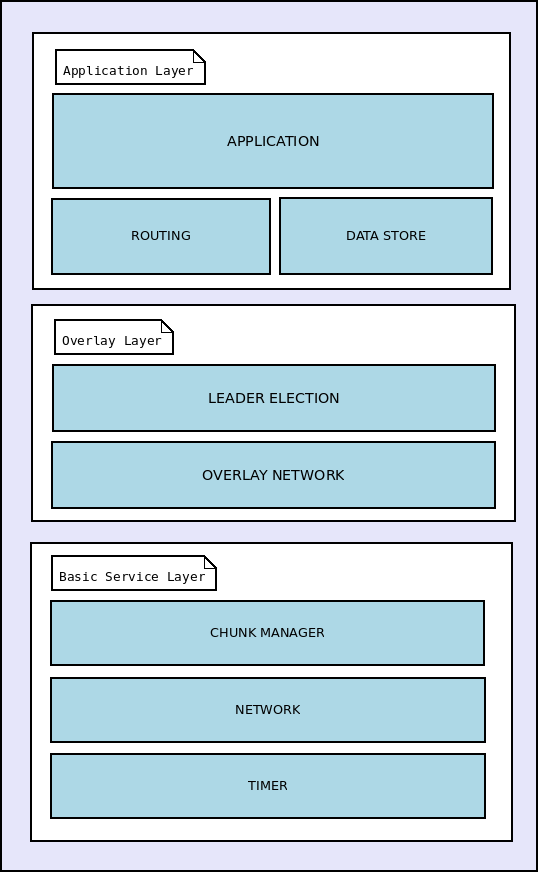
\includegraphics[width=8cm, height=12cm]{architecture_new}
	\centering
	\caption{Architectural Overview}
	\label{fig:architecture}
\end{figure}


%\begin{figure}[h]
%	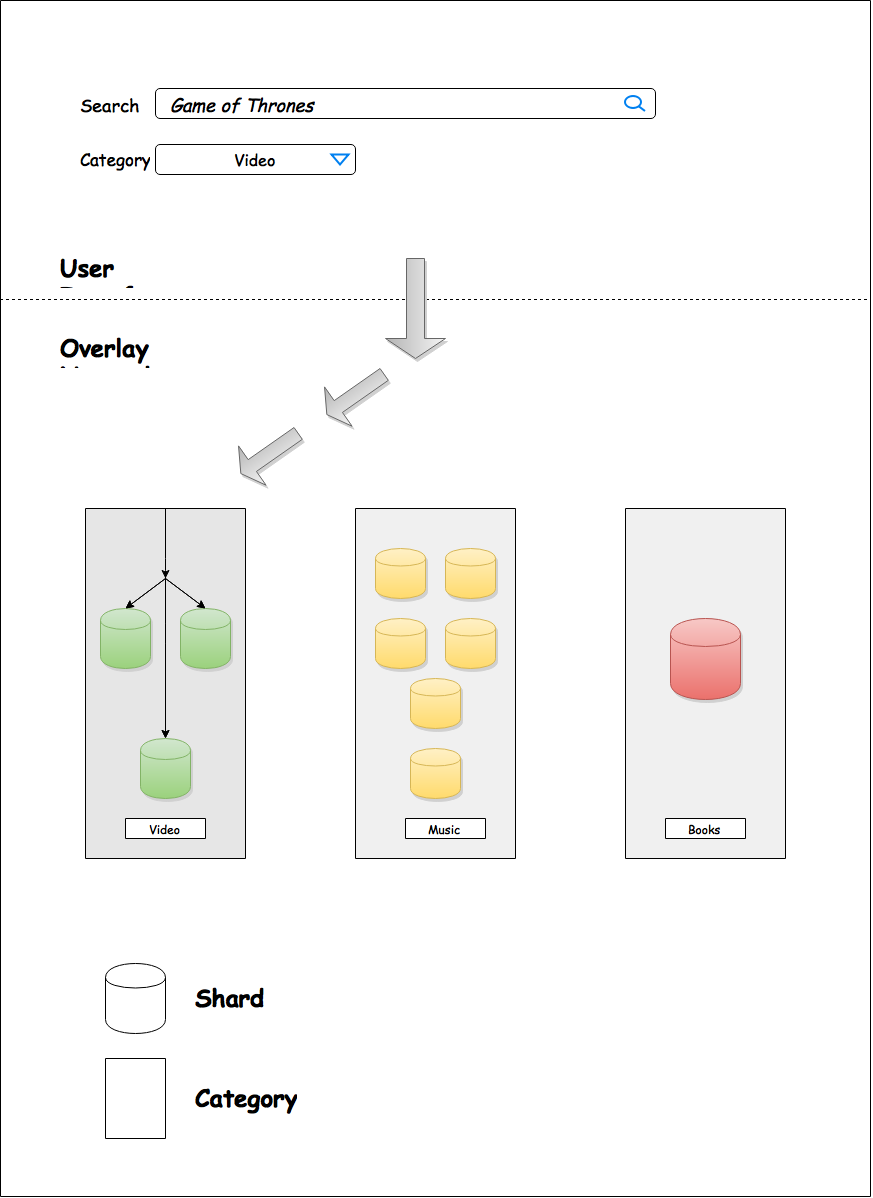
\includegraphics[width=10cm, height=12cm]{architecture}
%	\centering
%	\caption{Architectural Overview}
%	\label{fig:architecture1}
%\end{figure}

\section{Leader Selection Protocol}
\label{ssec:leaderElection}


In context of distributed systems, a lot of approaches regarding the leader election have been discussed. Most of the approaches involve all the nodes in the system to know and agree about a node being elected as a leader. This process of agreement between all the nodes works fine in case the nodes in the system are limited and known to each other but as the scale of the system increases, the approach of having agreement between all the nodes becomes unfeasible mainly due to the bandwidth utilization in terms of messages exchanged and also the time required to elect a new leader which increases dramatically. In addition to this, as the system needs to be deployed over open networks where nodes can join and leave as they want, the time to reach an agreement may increase further because nodes taking part in election might suddenly leave which will result in election round being discarded.
\par In order to make the leader election protocol suitable for Open Internet with churn, we modified the protocol to be a weaker variant of the existing algorithms and is known as \textit{Leader Selection Protocol}. The responsibility of electing a leader is now handled by a small group of nodes in the system. The group is decided by the node asserting itself to be leader and is known as follower group. The decision taken by this group is then communicated to rest of the peers in reasonable time. This process helps in reducing the message and time complexity for electing a new leader.



\subsection{Eventual Leader Election}

The leader election protocol developed as part of the thesis is a combination of the Paxos\cite{lamportPaxos}, Bully\cite{bully} and the Monarchical Leader Election\cite{guerraoui} algorithms. It resembles bully in terms of the node with the highest utility will try to enforce itself as the leader. In addition to this, in case the existing leader dies, the next best node in terms of utility will take its place thus resembling the Monarchical leader election. Finally, similar to Paxos, the leader selection algorithm also has :

\begin{itemize}

\item \textbf{proposers}: nodes which will take over leadership in case current leader dies.
\item \textbf{acceptors}: followers
\item \textbf{learners}: all peers.

\end{itemize}

The selection of the leader is performed by the nodes in the follower group. The information gets disseminated to rest of the nodes through a generic pull mechanism.

\subsection{Gradient Overlay}

As mentioned earlier, each node asserting itself to be the leader, selects its group of nodes with which it will initiate the selection protocol. The immediate problem that arises is the identification of this group. The gradient topology helps the node asserting itself as a leader to identify this group. The gradient topology is based on a preference function which helps each peer to choose its neighbors over the others based on the utility. The preference function used in the system helps the gradient topology to arrange the nodes with the higher utility towards the center of the system whereas the nodes with low utility are present towards the edges of the system. The nodes with the utility lying in between the two are present in the internal structure between the center and the edges. The gradient topology helps to provide a total order on the nodes. Ideally the node at the center of the gradient initiates the leader election protocol and it chooses the follower group to be \textit{topK} nodes where K is the size of the follower group.


\subsection{Overlay Stability}

The overlay is said to be stabilized once the change in the neighbors of a particular node is below a certain threshold. During the lifetime of the system, new nodes can join the system while existing nodes can leave it thereby resulting in churn. In addition, the utility of nodes can change which enables them to move in the gradient. Therefore, it might result in the the overall gradient topology being destabilized. In this situation, each node locally determines the stability of its neighbors by starting a convergence counter. On every shuffle round where each node updates its neighbors, the counter gets incremented in case the change in the view as compared to the previous view is below a predefined threshold. In case the change is more than the threshold it forces the node to reset the counter. The convergence counter enables each node to determine the local stability of the gradient as each node has only a subset view of the whole system. A node can initiate the leader election protocol when the counter reaches a defined value.

\subsection{Protocol Overview}

Each node in the system periodically executes the leader code shown in Algorithm \ref{leader} and also the follower code as depicted in Algorithm \ref{follower}. As part of the leader code, the node checks if the conditions for being the leader holds. In case the conditions are satisfied, the node initiates a voting protocol to the \textit{topK} nodes in the system known as the follower group. On receiving the voting request, the follower code gets executed. It checks whether the node deserves to be the leader and in case all the conditions are fulfilled, it sends back as acknowledgement. Only on receiving the acknowledgments from all the nodes in the follower group will the node finally assert itself as the leader and initiates a lease at its own end and informs the follower group about the lease and the new leader round.
\par The leader uses its followers to replicate the decisions taken in order to ensure redundancy. After expiry of every lease, the leader will again check if conditions for it to be the leader holds. In case the conditions are not met, the leader stops with the lease extension. The lease eventually expires at the followers group and they again wait for a new leader to emerge.


\subsection{Utility Values}


In this section we will be giving a brief introduction concerning the parameters used by the different nodes to calculate their utility. It is explained in greater depth in the Section {ref:utility}. The nodes arrange themselves in the overlay based on the utility, with the higher utility ones getting concentrated at the center of the system. The utility is decided based on following parts:

\begin{itemize}

\item \textbf{leaderGroupMembership}: boolean value indicating that the node is part of either a leader or part of follower group.  The check gets enabled when the node either gets elected as a leader or becomes a part of the follower group. This ensures that the follower group remains as the \textit{topK} nodes during the lease round as the nodes joining the system or already present will have the check being disabled. This check if enabled provides a boost to the utility of the node ensuring they remain at the center of the gradient.

\item \textbf{replicationScore}: The decisions that are taken by the leader which have been replicated by a particular node.

\item \textbf{peerScore}: It represents score of a peer based on its internal properties like bandwidth, processing capability. A node with a better peer score has capability to serve information to a larger audience.

\item \textbf{identifier}: The last is the \textit{identifier} of the node which is used as a tie breaker and provide total order on nodes.

\end{itemize}


\subsection{Leader Behavior}

The behavior of the leader is depicted in Algorithm \ref{leader}. The leader module in each peer checks the below conditions periodically to determine if the node needs to initiate the leader election protocol :

\begin{itemize}

\item \textbf{Leader Round Detection} : The node initially checks whether it is already a leader by checking if its \textit{leaderGroupMembership} variable is switched on or not. In case the node is already a leader, it doesn't initiate a new leader selection protocol.

\item \textbf{Local Gradient Convergence} : Next the node determines if the local gradient is stable and converged meaning that the rate of change of neighbors is below the defined threshold.

\item \textbf{Leader Rules Satisfied} : The node checks its gradient to locate a node better than itself in terms of utility. In case a better utility node is located, the current node backs off and does not initiate the leader selection protocol.

\end{itemize}

Once the conditions are met, the node initiates the voting process as part of leader election protocol. It selects topK nodes which will be part of  its follower group and sends them a promise request meaning that they accept the node as their leader. It then waits for their responses. Rejection from any node means that there might be a node which is better than the leader which has not yet been discovered by the leader itself. The leader then cancels the current election round and wait for the conditions to be met again before initiating the protocol.
On the other hand, if the leader receives promises from all the nodes in its follower group, it informs the follower group about it being elected as leader which results in nodes starting a lease for the current leader.  Before the expiry of the lease, the leader again checks if the conditions for itself to become a leader are met and in case the conditions hold, it informs its follower group about extension of the lease. The follower group at this point might not be the same as in previous round. The node recalculates the topK nodes before extending the lease and send them the extension request. In case the lease is not extended it expires and the node resets the leader group membership check.

It might also be possible that at the time of extension, the leader might discover a node which is better than the leader itself and in order to promote fairness in the system, the leader will not extend its lease anymore and allow the new node with better utility to impose itself as the new leader.


\subsection{Follower Behavior}

The behavior of the nodes in the follower group is depicted in Algorithm \ref{follower}. Each node in follower group accepts the promise request from the node in case it satisfies the below conditions:

\begin{itemize}

\item \textbf{Leader Round Detection} : The node checks whether it is already a part of follower group or has already promised to another node. If any of the mentioned case is true, the node rejects the promise.

\item \textbf{Leader Rules Satisfied} : The utility of the node that is requesting the promise has a better utility than utility of self as well as the nodes contained in the local gradient view.

\end{itemize}

In case the above conditions hold, the node sends an acknowledgement in regard to the promise request. The node then initiates the timer and waits for the commit request regarding the node being elected as leader. During this period, the node will reject promise request from any other node. The above condition also reduces the probability of emergence of two leaders simultaneously in case the follower group of the two nodes trying to elect themselves as leader overlap with atleast one node In case the event is not received before the timer expires, the node resets the condition and becomes ready to accept other promises. Once the node becomes part of the follower group it will switch on the leader group membership check and boosting its utility. It will also reject the promise request from any other node in this state.

\subsection{Lease Extension}



\subsection{Multiple Leaders}

The leader module on each node, checks whether the conditions for becoming a leader are met and in case the conditions hold initiate the leader election protocol. Ideally, based on converged system only a single node with the highest utility should initiate the leader election protocol and be chosen as the leader but under certain special circumstances multiple nodes can initiate leader election protocol and get elected as leaders. The links with which the nodes communicate with each are fair loss links and therefore can drop messages. It might be possible that a large number of messages are being dropped by the links and therefore two different nodes are unable to detect each other and start election protocol. As part of topK nodes that are chosen by the two nodes, even if a single node overlaps it would prevent the election of two nodes as leaders simultaneously but in case the topK group of nodes has no common member which can happen in event of network partitioning, the two nodes will be elected as two leaders. Once the network heals, they will detect the presence of the other and one of the elected nodes will give up leadership.


\subsection{Information Dissemination}

Once the leader gets elected the information about the new leader is initially present with the follower group. This information needs to be disseminated in the system to other peers. As each node in the overlay can reach the topK nodes in O(logN) time, the information gets pulled by the nodes near the center from the center and nodes lying away from the center pull the information from their parent provided to them by the gradient in logarithmic time.

\begin{figure}[h]
	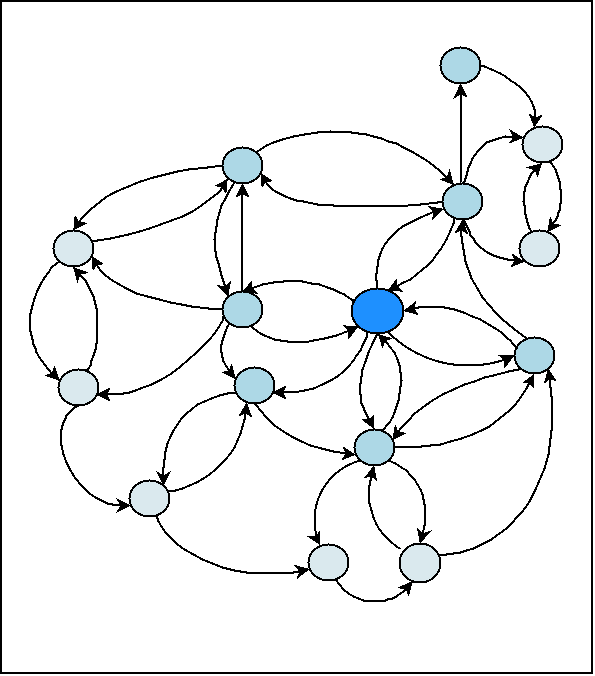
\includegraphics[scale=0.5]{p2p}
	\centering
	\caption{Peer Arrangement}
	\label{fig:p-arrange}
\end{figure}


\begin{algorithm}[h]
\caption{Eventual Leader Selection - Leader}
\label{leader}
\begin{algorithmic}[1]
\Upon[init]{nodeId}
  \State $selfId := nodeId;$ $round := 0;$
  \State $isLeader := false;$ $stableGradient := false;$
  \State $gradSample := \emptyset;$ $followerGroup := \emptyset;$
  \TriggerS[periodicCheck]{}\EndTriggerS
 \EndUpon

\Upon[gradientSample]{sample}
  \State $stableGradient := $ \emph{stable}$(sample);$
  \State $gradientSample := sample;$
 \EndUpon

\UponS[periodicCheck]{}
  \If{$!isLeader$ AND $stableGradient$ AND \emph{highestUtility}$(selfId, gradientSample)$}
     \State $followerGroup := $ \emph{getTopK}$(gradientSample);$
     \ForEach[followerGroup]{member}
       \Trigger[promiseReq]{selfId, round} \EndTrigger
    \EndForEach
    \TriggerS[roundTimeout]{} \EndTriggerS
    \State $promiseSet := \emptyset$
  \EndIf
 \EndUponS

\Upon[promiseAck]{pNodeId, pRound}
  \If{pRound = round}
    \State $promiseSet := promiseSet \cup \{pNodeId\}$
    \If{followerGroup = promiseSet}
      \ForEach[followerGroup]{member}
        \Trigger[lease]{selfId}\EndTrigger
      \EndForEach
      \State $isLeader := true;$
      \TriggerS[leaseTimeout]{}\EndTriggerS
      \TriggerS[cancelRoundTimeout]{}\EndTriggerS
    \EndIf
  \EndIf
\EndUpon

\algstore{leader}

\end{algorithmic}
\end{algorithm}


\begin{algorithm}
\begin{algorithmic}[1]

\algrestore{leader}
\Upon[promiseNack]{pNodeId, pRound}
  \If{pRound = round}
    \State $round++;$
    \TriggerS[cancelRoundTimeout]{}\EndTriggerS
  \EndIf
\EndUpon

\UponS[roundTimeout]{}
  \State $round++$
\EndUponS

\UponS[leaseTimeout]{}
  \State $sample := $ \emph{resetUtility}$(gradientSample);$
  \If{\emph{highestUtility}$(sample)$}
    \State $followerGroup := $ \emph{getTopK}$(sample)$
    \ForEach[followerGroup]{member}
      \Trigger[lease]{nodeId} \EndTrigger
    \EndForEach
    \TriggerS[leaseTimeout]{}\EndTriggerS
  \Else
    \State $isLeader := false;$
  \EndIf
\EndUponS

\end{algorithmic}
\end{algorithm}

\begin{algorithm}[h]
\caption{Eventual Leader Selection - Follower}
\label{follower}Disadvantages
\begin{algorithmic}[1]

\UponS[init]{id}
  \State $isFolower := false;$
  \State $selfId := Id;$ $pendingPromise := Nil;$
  \State $gradientSample := \emptyset;$architecture
\EndUponS

\Upon[gradientSample]{sample}
  \State $gradientSample := sample;$
 \EndUpon

\Upon[promiseReq]{nodeId, round}
  \If{$!isFollower$ AND $pendingPromise = Nil$ AND \emph{highestUtility}$(nodeId, gradientSample)$}
    \State $pendingPromise := nodeId;$
    \Trigger[promiseAck]{selfId, round}\EndTrigger
    \TriggerS[promiseTimeout]{}\EndTriggerS
  \Else
     \Trigger[promiseNack]{selfId, round}\EndTrigger
  \EndIf
\EndUpon

\UponS[promiseTimeout]{}
  \State $pendingPromise := Nil;$
\EndUponS

\Upon[lease]{nodeId}
  \If{$pendingPromise = nodeId $}
    \TriggerS[followerLeaseTimeout]{}\EndTriggerS
    \TriggerS[cancelPromiseTimeout]{}\EndTriggerS
    \State $isFollower := true;$
    \State \emph{setFollowerUtility}$();$
  \EndIf
\EndUpon

\UponS[promiseTimeout]{}
  \State $pendingPromise := Nil;$
\EndUponS

\UponS[leaseTimeout]{}
  \State $isFollower := false;$
  \State \emph{resetFollowerUtility}$();$
\EndUponS

\end{algorithmic}
\end{algorithm}





\subsection{Preference and Utility Function}
\label{ssec:utility}

Gradient Topology is a class of P2P topology which helps in constructing the overlay of the system in such a way that the nodes with higher utility are concentrated at the center and the nodes with low utility are present on the edges of the system. The topology makes use of the utility function which is a system based function used to achieve total order on the nodes. As per the current system, the utility function is composed of four scalars:

\small
\begin{equation*}
    LeaderGroup \prec ReplicationScore \prec PeerScore \prec PeerID
\end{equation*}
\normalsize

The parameters contained in the utility function are used to provide score to each peer in the system. In order to compare the utilities of two different peers, we start comparing the parameters mentioned above in direction from left to right. In case the outcome cannot be decided by a particular parameter comparison, the comparison moves to the next parameter. The tie breaker is the last parameter i.e. peer identifier. In order to better understand the utility function used in the system, we will be providing brief description about the parameters used:

\begin{itemize}


\item \textbf{leaderGroupMembership}: It is a boolean check which indicates if the node is a leader or part of the follower group. Once the node becomes part of follower group, it switches on the check which provides a boost to its utility as compared to other nodes in the system which are not part of the follower group. This parameter is chosen as the first in comparison because once a peer gets elected as the leader and chooses its follower group, it needs the group to be stable and be in the topK in the system.


\item \textbf{replicationScore}: The next parameter in comparison is the replication score which is a numerical value indicating the decisions that are taken by the leader and which have been replicated by the node itself. As the system evolves and new information gets added or updated by the leader, these decisions are also replicated at other nodes in the system. A node with higher value of replicationScore is better suited to take  over leadership in case the leader crashes because it would have replicated most of the decisions taken by the leader and information loss if any would be minimized.

\item \textbf{peerScore}: The peerScore is another parameter having a numerical value indicating the capacity of the node to serve audience in the system. The nodes which have higher bandwidth, computational and storage capacity have a better chance to serve a wider audience in terms of information dissemination. The score regarding the computational and storage capacity, bandwidth and session time gets aggregated and represent the peer score. Therefore, these peers have a higher peer score and should be located near the center of the overlay.


\item \textbf{peerId}: This parameter is used to represent the identifier of the peer.  It is based on the assumption that all the nodes that join the system, do that with a distinct identifier. It used as the tie breaker in case all the values before are unable to decide a peer with better utility and therefore the last in the comparison order. As part of system, a node with a lower value of identifier has a better utility as compared to a node with same parameters but a higher identifier.

\end{itemize}


The total order achieved on the nodes using the utility function is used to assign ranks to the nodes with the leader with the highest utility being assigned a rank 0. Therefore, in a system with N nodes, N ranks are being assigned. The main reason behind assigning ranks is the creation of fingers which are long range links used as paths for faster dissemination of data. A node with rank R will try to create fingers i.e. links with nodes with ranks near to value ( R / 2 ). Once these links are created, node periodically gossips with the long range links to refresh the links in case the nodes behind the fingers have crashed. As there is no centralized control in the system, the mechanism to estimate self rank is based on the ranks of the neighbors of a particular node. Initially each node starts with self rank as $ \infty $. In case a node is unable to find any node above itself in terms of utility, it resets its rank as \textit{zero}. Each node then identifies the minimum rank among the neighbors [R1 .. RS] of size S, it then calculates its own rank by MinRank(R1, R2, ... RS) + diff  where \textit{diff} is number of neighbors who are better than the node in terms of utility. As the neighbors keep on changing due to churn and updation of self utility, so does the rank keep of changing. Ideally, the node with rank zero initiates the voting protocol.

\begin{figure}[h]
	\centering
	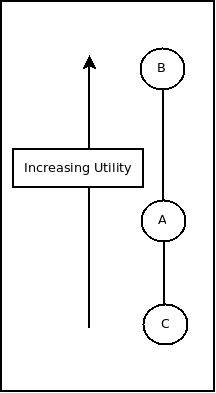
\includegraphics[scale=0.5]{preference}
	\caption{Utility Scale}
	\label{fig:preference}
\end{figure}

\par The gradient topology constructs and maintains the overlay by forming links with a set a preferred nodes in the system. The gradient also selects a node from this set and exchange information regarding the change in the self utility and neighbors periodically. In order to decide the set of preferred nodes, gradient uses a \textit{Preference Function} which itself is based on the utility function. In the prototype developed as part of thesis, the preference function indicates that a node will have a higher preference to form link with the node having a utility higher but closer to a node's own utility. In case a node is unable to find nodes above itself in terms of utility it will form links with node that have a utility which is lower than self but closer to self. In order to better explain the statement, we assume that we have three peers having identifiers as A, B and C. Assuming the utility of a peer could be represented on an absolute scale as depicted in Figure \ref{fig:preference}, we can see that PeerB has the highest utility  followed by PeerA and then by PeerC. The preference function indicates that PeerC will have a higher probability of forming link with PeerA than with PeerB as even though both have utility greater than its own, PeerA has utility which is closer to utility of PeerC. \textit{Softmax} approach is being used with a \textit{low temperature} to identify the nodes that will be part of the neighborhood list resulting a greedy approach while creating the local view. Apart from this, gradient also uses the  preference function while selecting a node from the neighbor list to shuffle with from the local view. At this stage, the softmax approach with a \textit{higher temperature} is used to increase the range over which the node is selected for shuffling.


\subsection{Pull Protocol}

The whole system is managed by a small number of peers which are the leaders of different shards in the system. The protocol employed for election of leader is \textit{Leader Selection} which is explained in detail in section \ref{ssec:leaderElection}. The leader is responsible for taking decisions regarding addition or updation of entries in the shard. In order to make the system highly available and prevent a single point of failure, the leader replicates the decision over the follower group. Once the decision has been replicated to the follower group, the leader returns back a successful response to the client which initiated the operation. This decision needs to be disseminated to other nodes in the shard which can be achieved by either using a push protocol in which nodes send information to their neighbors or through a pull protocol, which is periodically executed by each node and asks for any updates from the nodes having higher utility. The push protocol seems lucrative because the nodes will push information to other nodes only when a new information gets available to them. It prevents the nodes from periodically requesting for any new information from the neighboring nodes and thus saving bandwidth. But there are major flaws in the push information scheme which are enumerated below:

\begin{enumerate}

\item From the security point of view, the push protocol is vulnerable to the Byzantine node attack. In case a node gets compromised, it can start pushing junk data to other nodes.


\item As the system is dynamic, nodes can arrive and leave the system at any time. A simple push protocol, prevents the node just joining the system to get all the updates pushed by the nodes higher in the utility prior to its joining.

\item A big flaw in using push protocol for the current prototype implementation is the way in which the preference function is defined. As mentioned earlier a particular node prefers node which higher but closer to itself in terms of utility. Therefore, given enough peers present above a particular node in terms of utility, that node will form all the neighborhood connections to the peers above itself. This tendency prevents nodes forming links with the peers on the edges of the shard i.e. the nodes having low utility. In absence of links, there is a high chance that the updates pushed by other nodes won't reach the nodes lower in the gradient.

\end{enumerate}

Therefore, when the information needs to be disseminated in whole of the system, a pull protocol is employed whereby every node periodically requests for the next decisions that are taken by the leader and not yet seen by the requesting node. Apart from this, the system involves the use of push protocol by the leader when the decision needs to be replicated to the follower group. The information gets pushed by the leader to the nodes in the follower group which gets pulled by the rest of the nodes in the system using a pull protocol. Even though we have briefly talked about information dissemination in this section, it is explained in detail in Section \ref{ssec:gossip}.

\subsection{Gossip Based Data Dissemination}
\label{ssec:gossip}
Once a node becomes a leader, it is implicitly trusted by other members in the shard. Initially the information of a node becoming a leader is only published to the follower group which is chosen by the leader. This information then gets pulled by other peers in the system. In this situation, it might be very much possible that a Byzantine Node might start publishing wrong information to the peers during the pull protocol. In order to prevent this, a peer during the pull protocol, requests updates from a predefined configurable peers usually \textit{three} that are above itself in terms of utility.  The peers respond with the hashes of the information. Only the information for which the hashes match from all the nodes is then pulled from any one of the responding peers.
\par This approach is being used for securely disseminating the leader information in the system. In addition to this, entry dissemination is also based on this protocol. We think that this approach is secure enough in the sense that it is highly unlikely for all the nodes that are requested by peer to provide updates that are faulty.


\subsection{Load Balancing}
\label{ssec:loadBalance}
As the system evolves, the leader receives request for adding new entries in the system. Using basic replication strategies, the leader commits the entries to the leader group which then gets replicated to all the nodes in the shard using pull protocol. The system has a predefined \textit{MaxShardSize} parameter. When the entries grow beyond the count, the leader then initiates \textit{ShardSplit} protocol. As part of this protocol, each peer based on its identifier and its depth which is basically number of shard splits seen by the node, decides the next shard id.
\par Before initiating the two phase commit of the shard split, the leader stops handling the entry additions. It then looks in its local lucene store and after sorting the entries based on their identifiers, calculates the split point. This meta information is then committed to the leader group nodes along with the shard split update as a part of two phase commit. Once the information is pulled by other peers in the system, based on their new shardId, they decide to remove all the entries either before or after the split point. The process of removing the entries in more detail when we introduce the concept of Leader Units and Timeline in section \ref{ssec:leaderUnit} and \ref{ssec:timeline} respectively. The peers then join the other peers in their respective shards.



\subsection{Routing}
\label{ssec:routing}

\par The client in order to look for the entries in the system generates a search request. The search request is then sent to the application running at the client node. The protocol of handling search request by the application involves locating the items matching the search request in the local data store. Once the matching items are located, necessary information is extracted from the items and response is generated to be sent back to the client.

\par The above approach allows application to locate all the matching items in case all the data is located in the local data store. As part of load balancing protocol which explained in Section \ref{ssec:loadBalance}, the data gets distributed between the nodes in different shards. Now, it might be possible that the item that the client is looking for is located in other shards. Therefore, the application now needs to route the request to the nodes present in these shards. In order to do so, the application needs to have information about the shards and sample of nodes located in each shard. Therefore, each peer has a \textit{Routing} abstraction which keeps track of the shards in the system and sample of nodes inside each shard. The component periodically gets random set of samples from the peer sampling service. Each node sample contains information regarding the shard to which it belongs. Using this information, the component maps the node descriptor to the shard. Now, when the application receives a search request, it gets information about all the shards and a set of descriptors in each shard from its local map. The query is then sent in parallel to all the shards.




\chapter{Implementation}
\label{chap:impl}

In order to check for the viability of the theoretical approach, we worked on developing a prototype on the principles stated in the design section. The prototype used Apache Lucene for storing and indexing data. In addition to this, the prototype was developed using the Kompics framework which is an asynchronous message passing system. The main application process on each node in the system is composed of following abstractions: \textit {group membership, routing, leader election} and \textit{data storage} abstraction. All the modules interact with the \textit{network} and \textit{timer} abstraction which are used to send messages over the communication network and configure local timeouts respectively. In addition to this, we have a \textit{message chunking} abstraction which as name suggests check the messages going over the network and in case the message exceeds the maximum transmission limit, fragments the packet and at the receiving end joins the fragments to construct the final message. All of the abstractions are built from scratch in Java and have been previously explained in greater detail in Section \ref{sec:architecture}.

\par A high level view of the interaction of a single user layer with the system layer is shown in Figure \ref{fig:overall_function}. In case a node receives a request for adding an entry in the system, it forwards the request to the application module. The module initially checks whether the node is the leader for the current shard. In case it is the leader, it invokes the entry addition routine on self. Otherwise, it sends the request to the routing module to route the request to the leader. As part of current implementation, the entry addition routine is a synchronous operation which involves performing a two phase commit by the leader over the nodes constituting the follower group. Only when the leader receives responses from the majority of follower group nodes, it commits the entry locally. In order to commit the entry, application module interacts with the data module to add the entry in the lucene. Once the entry gets replicated, the leader responds back to the node from which the request originated.

\par Apart from this, the prototype developed allows the user to search for the entries added in the system. The \textit{Search Entry Operation} involves user entering the name of the document to be located. The middleware constructs a well defined search pattern which is understood by the lucene in the data storage abstraction. The search request is initially handled by the application module of the client. The application module sends this request to the routing module to check for the references of the nodes located in different shards in the system which are populated by the gossiping protocol constantly supplying random subset of the global samples to the routing module. The module then routes the request to nodes in each shard. As the number of shards can grow, it can easily result in large fanout search causing a long tail. To prevent this, we route request to more than one node in each shard and only handle the response from the fastest node and reject the other responses. The search responses are added in a separate lucene instance. In case all the shards responded or the timeout for search operation, whichever gets triggered first, the responses are then sorted and returned back to the client.


\begin{figure}[h]
	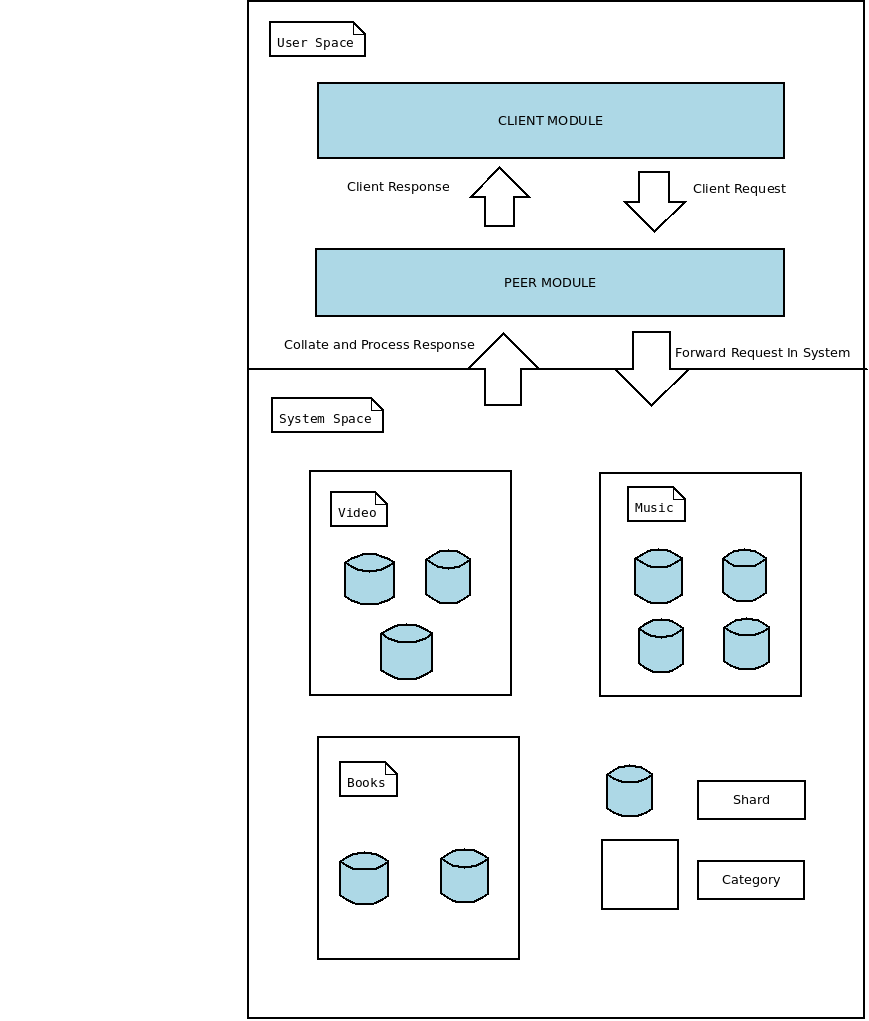
\includegraphics[scale=0.38]{OverallFunctioning}
	\hspace*{-5cm}  
	\caption{Architectural Overview}
	\label{fig:overall_function}
\end{figure}



\subsection*{Overlay Network}

The system strives to be a dynamic system in which the nodes can join and leave depending upon their requirement. Gradient topology built over peer sampling service is being used to construct the overlay of the system. The nodes perform shuffling as part of construction of a random graph and overlay is constructed using gradient topology over the random graph using preference function. Each node holds only a subset of total nodes which are known as \textit{preferred nodes}. The mechanism to identify the preferred nodes depends upon the topology. The application holds two different set of preferred nodes, identified under the gradient and the peer sampling service. Each service keeps on updating the set by periodically identifying a node based on different policies and initiate a shuffle with that node. As part of shuffle, nodes exchange a subset of the view held by them and merge in their local view the sample received from the other nodes. In this way, each peer is able to discover new peers joining the system. In addition to it, each sample also has an age attribute which gets incremented on every shuffle and helps to identify how long that particular sample has been in the system.

\par  As a node leaves the system voluntarily or by crashing, the sample of node in the system becomes stale. As an effort to keep neighborhood samples fresh, in case the size of the sample list grows beyond a predefined threshold, we removed the oldest sample i.e peer reference with the highest age. We quickly realized that if this approach needs to be successful, we would need to synchronize the rate at which the gradient and the peer sampling service performs shuffling with the neighborhood nodes. In case the difference between the shuffling rates of both the services is large, the outcomes of the stabilization of the gradient were unexpected. The main reason behind it is that the peer sampling service feeds the sample to the gradient service. So in case the rate of shuffling in the sampling service is fast, the increment in the ages would be frequent because as part of shuffling the peers increment the age of the references and then exchange sample. Therefore the sampling service will feed the samples with high ages and the gradient shuffling is at a lower rate resulting in the slow rate of increase in ages. The nodes disseminate their updated utility in the system through the shuffles with age \textit{zero}. Therefore, the node sample with a lower age would mean that it recently has been shuffled by the host node in the system and therefore indicates recent utility of the node. In case of difference in shuffling rates of the services with the sampling service shuffling faster than the gradient service, the probability of peer reference samples having ages higher than the corresponding samples present in the gradient sample is higher even though the peer reference from the sampling service has updated utility. Thus, the updated peer reference sample gets disseminated in the system slowly as the sample recent utility has a higher age than the same sample with old utility.

\subsection*{Operations}
As part of current implementation, the prototype supports the following operations:

\begin{itemize}

\item \textit{add-entry (name, category, description, date)}
\item \textit{search-entry (name)}

\end{itemize}


\section{System Data Structures}

In large scale distributed systems, \textit{availability} is achieved through data replication while the \textit{consistency} is achieved using Eventual Consistency strategies. The updates to an object are committed on a single node and then executed in the background on other nodes containing the replica of the object. This makes the system vulnerable to conflicts arising out of concurrent operations on different nodes which needs to be manually resolved or rollback of the updates needs to be performed. Marc Shapiro et al formally introduced the concept of \textit{Conflict Free Replication Data Types} \cite{crdt} \cite{crdtConcurrencyWithoutControl} which  enables the concurrent updates which commute to be executed on the replicas of an object on different nodes which can eventually be resolved locally without consensus. In addition to this, the author introduced the concept of \textit{Dense Identifier Spaces} required to identify the commutative concurrent operations \cite{crdtConcurrencyWithoutControl}. The entry identifier and other related data structures used in the system are motivated by the concept of these \textit{dense  identifier spaces}.


\subsection{Entry Identifier Structure}
\label{ssec:entryIdStructure}

The structure of the identifier used by the system to identify the entries is mainly composed of three parts which will be briefly explained in this section:

\begin{tcolorbox}
\textbf{Identifier Structure:} \textless Epoch, LeaderId, EntryId \textgreater
\end{tcolorbox}

Whenever a client receives a request for entry to be added to the system, the request gets routed to the leader of the shard and the leader of the shard based on its own local state determines the identifier with which the entry will be added in the system. Therefore, whenever a peer is chosen as a leader it will first identify different parts of the entry structure.
\par Whenever a peer becomes the leader of the shard, it firstly identifies the epoch part of the entry structure. The \textit{Epoch} is simply a counter which is incremented by the node when it is chosen as leader. So whenever a peer is chosen as leader of the shard, it looks into its data store and identifies the epoch counter of the previous leader. In case if the node is the first leader in the system, the value of the epoch counter chosen is \textit{zero}. Otherwise, the peer increments the epoch of the previous leader by one. In addition to this, it also performs a commit over its follower group to inform them about the epoch with which it will be adding entries in the system.
\par As part of current implementation, each leader will start adding entries under a particular epoch with the \textit{EntryId} part starting at \textit{zero} and being incremented on subsequent adds under same epoch. In addition to this, each node uses its own identifier which it gets at time of joining the system after booting up as the value for the \textit{LeaderId} part of the entry structure.  An invariant that we maintain is that each peer joins the system with a different identifier. Therefore at any given time in the system, there won't be any two nodes with the same  identifier. The reason behind the invariant is that the identifier of the node act as tie breaker in the preference function explained in detail in Section \ref{ssec:utility} and which is used to provide total ordering on the nodes.

\par The main reason behind auto-increment of the entry id is to enable the nodes below in the system to identify the next entries to look for in the system. For example, if a node has already pulled an entry with entry id part of the entry structure as \textit{X}, it knows that the next entries for the particular epoch will be having entry identifier as \textit{X+1, X+2} and so on. Apart from this, the overall structure of the entry as a whole is chosen as to enable the creation of dense spaces. The requirement of dense space arise because of the issue of network partitioning. In a dynamic system which aims to run at hundreds of commodity machines, at any given time the nodes might be failing or the switches between the components might be broken. It can very well result in a network partition. As the system is self stabilizing, the nodes in the other partition will elect a new leader and evolve accordingly. When the partition heals and merge happens, we can now easily merge back the entries added in both the partitions because of these dense spaces. In order to better understand this, we can look at scenario in which there is a case of network partition and the each partition has elected its own leader. Let's say the identifier of two leaders are \textit{X and Y}. We also assume that both the leaders are operating in epoch \textit{E}. The entries added in this epoch are assigned entry identifier  incrementally starting from zero. Each leader starts committing the entries with a particular entry id which gets incremented on every subsequent entry add. Now when the network partition heals, we will have two sets of entries which can easily have the same epoch and the entry identifier value. In this case the presence of leader identifier in the entry structure ensures the uniqueness of each entry because the node which acted as leader can only be present in one of the partition. This scenario helps to establish the usefulness of the entry structure being used for the prototype. Figure \ref{fig:timelineMerge} presents the case of partition merge.

\par In above paragraph, we have identified the importance of the leader identifier and the entry identifier parts of the entry structure. In this section, we will be briefly mentioning the importance of the epoch identifier. The main use of the epoch identifier is help the system evolve with time. As new nodes gets elected as leader, they start adding entries with epoch identifier which is the increment of the epoch identifier of the previous leader. This process helps the system to identify the next entries to download once they have finished downloading the entries for a particular epoch. This nodes know that the next entries after the current epoch \textit{E}, if present will be with the epoch \textit{E+1}. Therefore, they start requesting the entries with the epoch \textit{E+1}. In this way, the nodes perform epoch switch and moves forward in the system.


\subsection{Leader Unit}
\label{ssec:leaderUnit}

A collection of entries added by a leader in a particular epoch is termed as a \textit{Leader Unit}. Each leader within a particular epoch can add only a specified amount of entries. As the number of entries reaches the threshold, the leader needs to perform a mandatory epoch switch. The structure of the leader unit is presented below:

\begin{tcolorbox}
\textbf{Leader Unit Structure:} \textless Epoch, LeaderId, NumEntries, State \textgreater
\end{tcolorbox}


The \textit{EpochId} represents the epoch under which the leader takes decisions in the system. The \textit{LeaderId} identifies the leader of the shard during that particular epoch. The \textit{NumEntries} part of the structure identifies the number of entries added by a particular leader. The value of this parameter can be below the threshold in case the leader crashes before the unit is complete but it can never exceed the threshold. Lastly, \textit{State} represents whether the leader unit is currently \textit{Open or Closed}. In case the leader is alive and taking decisions in the system, the state of the leader unit is \textit{Open}. In case the leader crashes or the threshold has reached for a particular leader unit, the unit needs to be \textit{Closed} either by a new leader or the same leader performing epoch switch.

\par We limit the entries that a leader can add in an epoch to achieve a balanced load distribution in newly created shards after sharding operation. As already explained in the section \ref{ssec:loadBalance}, during sharding phase, the leader calculates the split point identifier. It then performs a two phase commit over the follower group which gets pulled by other peers in the system. The split point is just used to identify the leader unit which will actually act as a splitting point. We never remove the entries within the leader unit instead we keep or remove whole of the leader units. In order to keep things simple, each node based on predefined bitwise manipulation algorithm identifies whether the leader units less than the split point needs to be removed or split point leader unit and higher needs to be removed. The minimum load on the system before the leader initiates sharding protocol is \textit{ X * Max Leader Unit Entries} where X is a configurable number.



\subsection{Marker Entry}

Although the concept of peer informing the follower group about the current epoch on becoming the leader of particular shard has been introduced in previous sections, we will briefly explain the process in this section.

\par Before a leader can start committing entries in a particular epoch, it needs to inform the other nodes in the shard about the epoch switch. The leader needs to make a \textit{marker entry} commit which will indicate the other nodes about the starting of the new epoch. The marker entry commit in addition of containing the information about the current epoch also contains the maximum number of entries added by the leader in the previous epoch. The current leader analyzes its local data storage module to calculate the entries added in the previous epoch. This information enables other node to close the previous leader unit with the number of entries specified. This information is committed to the follower group nodes which gets propagated to the system through the pull protocol.

\subsection{Timeline}
\label{ssec:timeline}

As the system is dynamic, any node can join and leave the system. In case the system has evolved enough and a new node joins the system, the new nodes also needs to pull entries from the neighboring nodes and evolve in the same manner to reach the stage at which the other nodes are present. Therefore the nodes in the system needs to keep track of the leader unit history. The timeline is an abstraction which mainly keeps track of the evolution of the system in terms of the order in which leader units added in the system. Based on the leader unit structure presented in Section \ref{ssec:leaderUnit}, these units are ordered based on the \textit{epoch identifier}.

\par At any moment in the system, the leader and the nodes in the follower group keep track of the latest updates to the shard in terms of entries being added or updated, leader unit switch happening because of the crashing of the previous leader or threshold regarding the entries that can be present in unit has reached and in order to continue the leader needs to perform a mandatory leader unit switch. In the system, knowledge regarding the leader unit is termed as \textit{Control Information} while the data added by the user is termed as \textit{Entry Information}. All the other nodes needs to periodically pull both the information from the nodes higher in utility using separate pull protocols which are briefly explained below:

\begin{enumerate}

\item \textbf{Control Pull Mechanism}: When a node joins the system, firstly the node needs to fetch the information regarding the in order leader units which are pulled as part of the Control Pull Mechanism. In order to pull the leader units, the base node requests the node above itself with the last leader unit as seen by the node during previous pull. In case the leader unit is \textit{Open} meaning the leader is still taking decisions as part of the unit, ideally the response should contain the updated leader unit else the response contains the leader unit with state as \textit{Closed} along with the next units that have added in the system. In case a node just joined the system, a special the request is made containing only an epoch identifier having value as \textit{zero}. The other nodes on seeing the request looks in there local timeline abstraction which is basically an in-memory leader unit list as shown in Figure \ref{fig:timeline} and calculates the next in order leader units based on the latest unit provided. The base node receives a list containing the next in order leader units and once the list is verified by the node, it sends the control information to the application.

\item \textbf{Index Pull Mechanism}: The application on receiving the control information, updates its local timeline with the information received. The Index Pull Mechanism contains the information regarding the leader unit which needs to be pulled by the node. Before initiating the entry pull, the mechanism requests any updates to the leader unit in terms of entries being added or the State of the unit being changed from Open to Closed. The mechanism also keeps track of the entries already being pulled. The mechanism requests for the next leader unit to pull in case the all the entries as part of the current leader unit have been pulled and the status of the leader unit has changed to closed meaning no new information will be added as part of the current unit.

\end{enumerate}

\par The leader units can contain maximum of \textit{N entries} or less which can happen because a leader can crash before completing the leader unit in which it was adding entries. Therefore the leader units added to the timeline can have different maximum entries. The application enforces the in-order pulling of the Control Information because in case a node is allowed to pull out of order leader units, any leader unit can be picked up by the index pull protocol in the application. In case the number of entries added as part of unit are large, it can result in the node's utility being increased in higher proportion as compared to nodes which are pulling in order and the units they are pulling have less entries being added as part of their unit. This might result for the node to start its own voting protocol and  become a leader for the shard. In case the node succeeds, it will be having entry gaps concerning the absence of in order leader units. It won't be able to pull it from any other node as the node itself is the leader and doesn't have any higher utility node. Therefore, we maintain the \textit{invariant} in which the \textit{timeline will not add and serve leader units out of order}.

\begin{figure}
	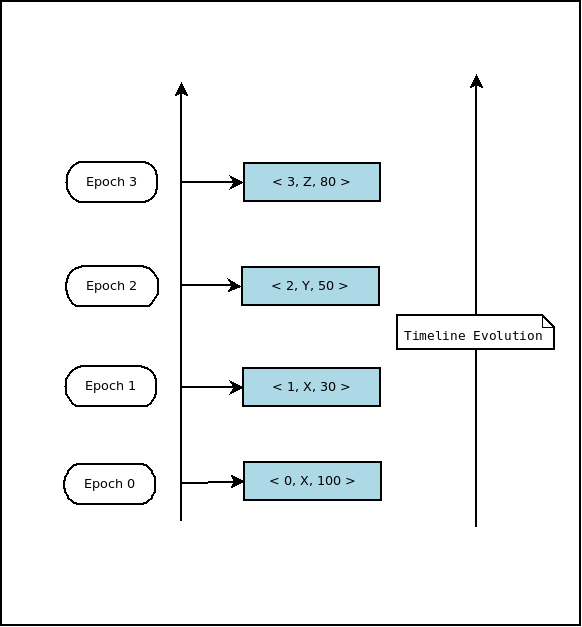
\includegraphics[scale=0.5]{timeline_new}
	\centering
	\caption{Timeline Evolution}
	\label{fig:timeline}
\end{figure}



\subsubsection{Skip Leader Units}

When a peer receives sharding update, the entry pull abstraction might currently be pulling a leader unit that is behind the sharding update or might have have already pulled all leader units before the sharding update. In any case, each peer gives priority to the sharding update. It pauses the current ongoing pull mechanism and analyzes the leader units that would have to be removed in case the node applies the update. Therefore, a node could realize that the leader units lying between the current unit that is being pulled and the sharding update are no longer required to be pulled as after applying the sharding update, these units would be removed.
\par The application needs to inform the entry pull protocol to skip some of the leader units. Therefore, each leader unit which is provided with a \textit{State} field which if set to \textit{Skip} will be jumped over by the entry pull protocol. The application updates the timeline by updating the leader units that needs to be skipped by setting the status to \textit{Skip}. Each peer has it's own set of leader units that needs to be skipped depending upon the units already pulled and units remaining between the last pulled and the sharding update. In best case scenario, the node could have pulled till the leader unit that will not be removed and the remaining ones needs to be Skipped. On the other hand, in worst case, a node could have already pulled all the leader units that would have to removed after sharding.

\subsubsection{Timeline Merge}
In section \ref{ssec:entryIdStructure} we introduced the concept of the dense identifier space created by the current identifier structure. In this section we will briefly explain the use of these dense spaces in event of network partition merge.


\par As mentioned earlier, at any given moment in data center the router, network connection between the systems or the switches might be failing. It could easily result in an event of network partition in which a group of nodes might get separated and isolated from the other group. The system prototype is supposed to be highly available meaning that the system should function correctly in event of network partition.

\par As it is not possible for the nodes to distinguish between the nodes getting partitioned or crashing, each group of nodes think that the nodes in the other group have crashed and they are ultimately removed from their view of system. The leader which was elected before the partition, keeps of functioning as the leader in one of the groups while the nodes in the other group realize about the death of their leader and start voting protocols to elect a new leader. Once a new leader gets elected, it chooses its own follower group and informs about the epoch under which it will be adding information in the system. In this way, the two groups keep on evolving separately without knowing about the presence of other group which is depicted in Figure \ref{fig:timelineMerge}.

\par Usually, the network partitions are short lived but in case of long lived partition usually manual intervention is required during the partition merge for the nodes in one group to discover the nodes in other group. In order to merge the two partitions effectively the leader units that were added since the partition in both the branches needs to be identified and added to the leader along with follower group of the merged partition, which would be pulled by other nodes in the system. The dense spaces created by the entry identifier structure allows entries added in two different branches to be identified uniquely. As we can see from the Figure \ref{fig:timelineMerge}, it is possible for the entries to be added in the two partitions with the same epoch and the entry identifier parts of the entry structure but the identifier of the leader that added the entries will be different because for a particular epoch, there could only be a single leader for a particular shard.

\par Once we identify the leader units that were added after the partition, they could easily be merged back in the timeline because of these dense spaces. Figure \ref{fig:timelineMerge} also depicts the above scenario of partition merge.



\begin{figure}
	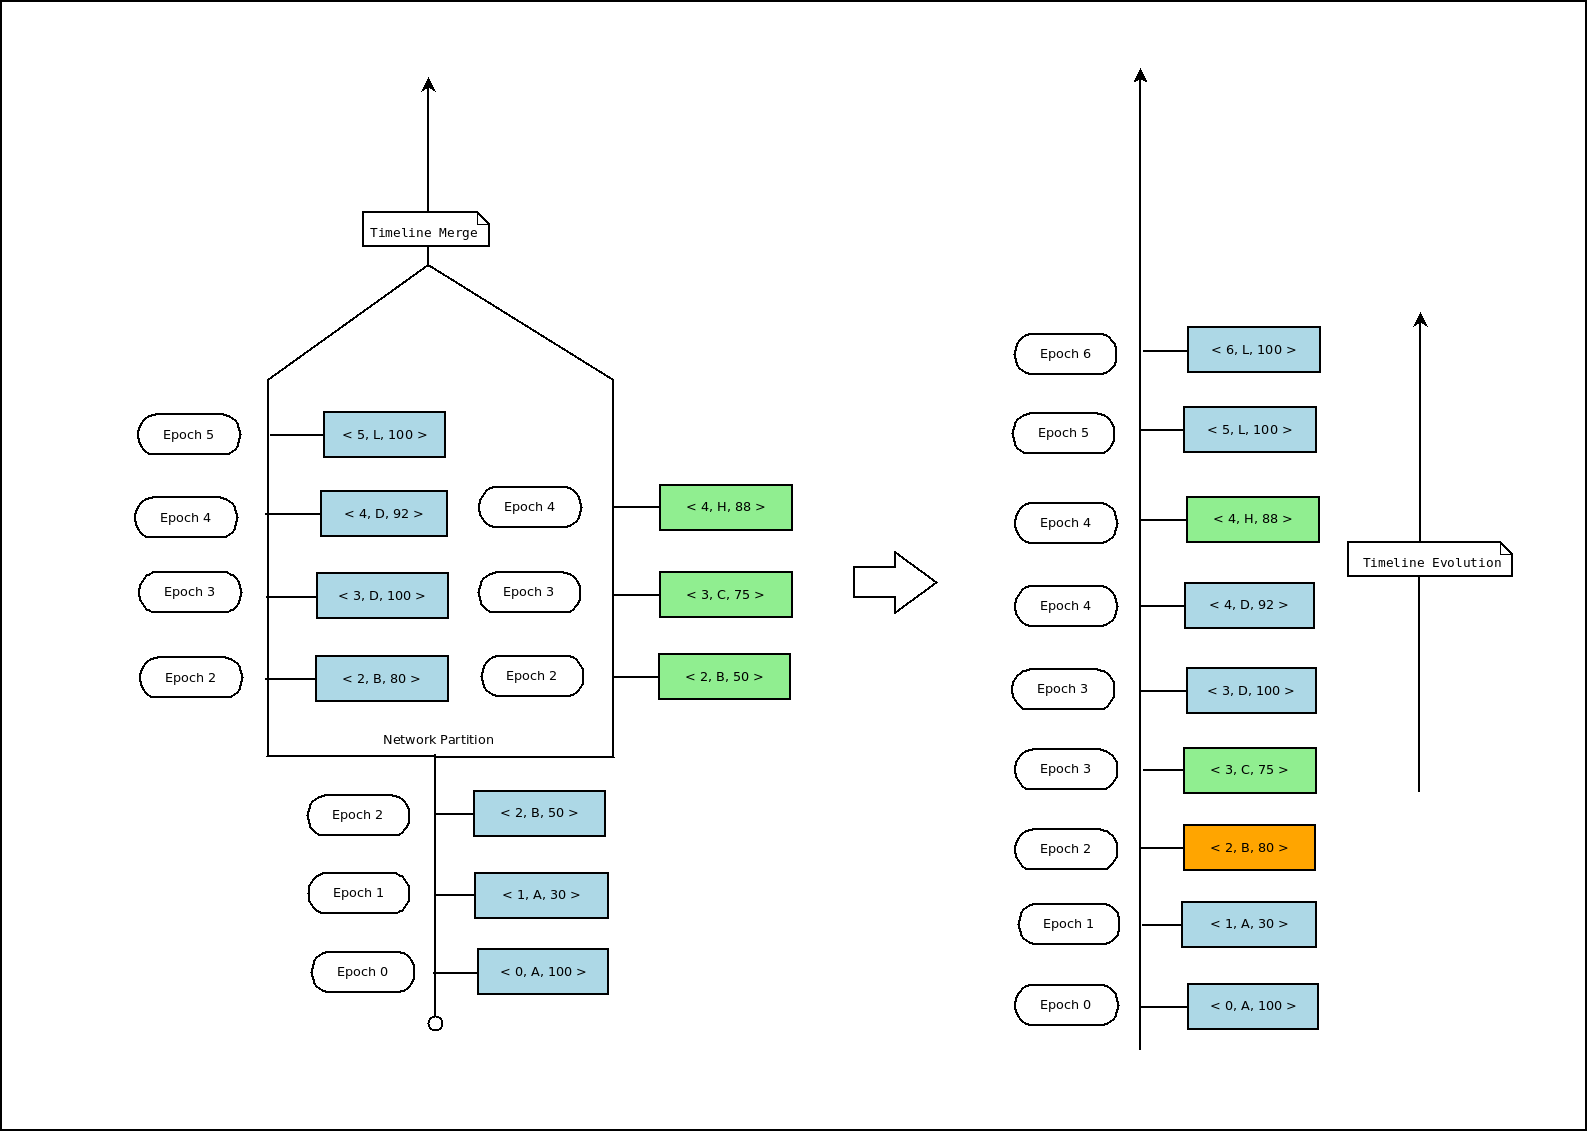
\includegraphics[width=14cm, height= 13cm]{timeline-merge}

	\caption{Timeline merge}
	\label{fig:timelineMerge}
\end{figure}


\newpage As we can clearly see from the Figure \ref{fig:timelineMerge}, a simple merge creates an issue of the \textit{split point leader unit}. When the networks split, the nodes in one of the partitions assumed the current leader to be dead and started their own election protocols while the leader being alive in other partition continued with its operation. This can be seen from the differences in the leader units having the \textit{same epoch} and the \textit{leader identifier}  but \textit{different entries} added in the system by the leader. When the partitions merge then the leader of the merged partitions needs to identify the presence of this case and needs to indicate the other nodes in the system to reopen the leader unit and fetch the remaining entries. The nodes which went into other partition than the leader at that time will recognize the difference in the entries and start pulling the remaining entries to become up to date.


\subsection{Request Fanout}

Earlier we introduced the concept of latency variability in large scale distributed systems and how it might be result in large response times. In the prototype developed, we analyzed different approaches for reducing the latency variability but
approach that we are interested and have adapted for our prototype involves sending the search request to multiple nodes within shard. We the application receives a search request from the client, the application locates the information regarding the nodes in the shard using the \textit{Routing} layer. We send the request to a configurable number of nodes within each shard and start a timer. We wait for the first response from that shard and discard the rest. The purpose behind it is to reduce the dependency on the slow performing node by replicating the request to other nodes within the same shard. Once, all the shards have responded or search request timed out, we collect, filter and augment the results with additional metadata. This data is then returned to the client. In this way the system makes significant steps towards preventing long tail in the search request response times.






\chapter{Evaluations}
\label{chap:eval}

In order to demonstrate the viability of the design of the system, we performed various experiments which will be discussed in this section.


\section{Experimental Setup}

The experiments were performed on the machine with the following specification:

\begin{itemize}
\item 8GB of RAM
\item Eight Cores (Intel(R) Core(TM) i7 CPU 860  @ 2.80GHz)
\end{itemize}

The prototype is developed in Kompics which is an event driven asynchronous framework written in Java. In order to achieve reproducible results, Kompics has single threaded simulation environment. As part of experiment a cluster consisting of several nodes is booted up in simulation on a single machine. A node in simulation resembles an actual deployed peer having its own separate component stack and address. As the nodes are on the same machine, the address of each node has similar IpAddress and port but different identifier. In order to communicate with the nodes during different phases of the simulation, a basic helper module is used to keep track of the nodes in simulation. A special node known as the \textit{leader node} is initiated with the lowest identifier value which enables the node to become leader during the initial leader election phase.

\par Apart from this, in order to monitor the health of the cluster as a whole, a special \textit{Aggregator Module} is built. As each node is composed of various components handling separate tasks, a \textit{LocalAggregator} component is introduced to aggregate the information at node level. This module periodically pushes the information to the \textit{GlobalAggregator} which as the name suggests stores the information from various nodes in the system. The aggregator at the global level also exposes option to register different processors to be invoked on the information aggregated. Depending upon the processor, specific information from the aggregated state is processed and different aspects of the cluster like average search response times, average entry replication lag etc. are analyzed.  


\section{Workload Setup}

The experiments are executed on a cluster of \textit{Two Hundred Nodes}, unless otherwise explicitly stated. In order to assure the reproducibility of the results, the Kompics simulation framework is inherently single threaded due to which the limiting factor concerning the scale of experiments is the strength of the processing unit of the machine.

\par Below is the list of the different parameters that were tuned for the simulations:

\begin{itemize}
\setlength\itemsep{0em}
\item \textit{gradientViewSize} - 10 nodes
\item \textit{croupierViewSize} - 10 nodes
\item \textit{gradientShuffle} - 1000 (ms)
\item \textit{croupierShuffle} - 1000 (ms)
\item \textit{branchingFactor} - 10
\item \textit{electionConvergenceRounds} - 6
\item \textit{electionConvergenceTest} - 0.8d
\item \textit{Entry Pull Round Timeout} - 4000 (ms)
\item \textit{Control Pull Round Timeout} - 3000 (ms)
\item \textit{maxEntryExchange} - 25 nodes/ pull
\end{itemize}

In addition to the above parameters, an important parameter is the minimum number of nodes that a particular node needs to locate above itself in terms of utility, to pull the control or the entry information. As part of the experiments, the value of the parameter is set to \textit{three}. This condition is respected by each node unless they are able to locate the leader in their local view. In event of presence of leader in their view, the nodes implicitly trust the leader and  directly pull the information from it.


\section{Convergence Experiment}

The \textit{Convergence Experiment} helps to understand the rapidness with which the entry gets disseminated in the system. As part of this experiment, we initially booted cluster with \textit{250 nodes} in simulation. Once the cluster was stabilized in terms of leader of the shard getting elected and the marker entry for the current epoch being published by the leader and disseminated to each node in the system, we then added a single entry to the leader and analyzed the time it took for the entry to be disseminated to all the nodes in the system. The results as shown in Figure \ref{fig:250conv} points out that it took 8 - 9 (sec) for all the nodes to get the entry. This time evaluates to roughly two pull rounds based on the value of the current pull round timeout.

\begin{figure}[h]
	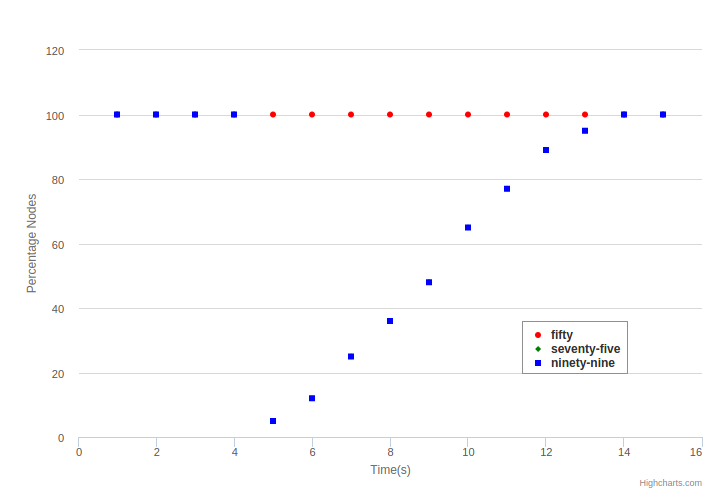
\includegraphics[scale=0.5]{250Convergence}
	\caption{Convergence - 250 nodes}
	\label{fig:250conv}
\end{figure}


Figure \ref{fig:500conv} shows the same experiment but now with \textit{500 nodes} in the simulation. The outcome is same as the previous one. The reason is because of the \textit{branchingFactor} parameter which is set to \textit{ten}. Based on the parameters for the current simulation, the top 600 nodes in the system are expected to receive the information within two pull rounds. The results of the experiment conform with the expected outcome.


\begin{figure}
	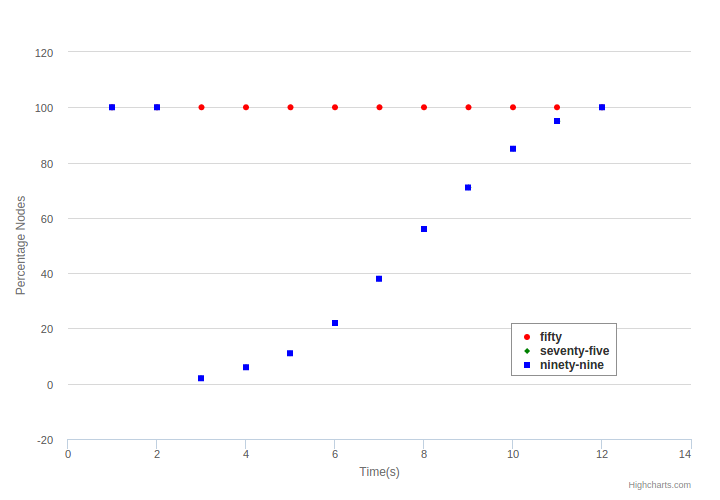
\includegraphics[scale=0.5]{500Convergence}
	\caption{Convergence - 500 nodes}
	\label{fig:500conv}
\end{figure}


\section{Add Entry Throughput}

As part of this experiment, we analyzed the response of the system under a constant rate of addition of entries. Based on the preference function, the nodes arrange themselves in such a way that the nodes with higher utility are concentrated towards the center of the system while nodes with lower utility arrange themselves on the outer regions of the system. Therefore, there is a gradient from the center to the outer edges of the system in terms of decreasing utility. In this experiment, we will be measuring the maximum lag in terms of entry difference between a particular node and the nodes in the follower group which ideally should have the maximum entries as the leader replicates the decision to commit a new entry over the follower group before adding the entry itself. The entry lag increases as we move towards the nodes in the outermost region in the system and therefore we would like to measure the maximum lag in fifty, seventy five and ninety percentile regions around.

\par We initially setup a cluster of 200 nodes in simulation. Once the system was stabilized, we added an initial batch of \textit{20 entries}. We then started adding entries at a constant rate for a fixed period of time. The experiment was performed  with the following variations:


\begin{enumerate}

\item We added the entries at rate of \textit{2 entries per second} for a duration of  \textit{100 seconds}. Figure \ref{fig:addEntry2} represents the maximum entry lag in different regions in the system.

\item As part of this variation, we increased the throughput to \textit{4 entries per second} keeping the duration same as before. Figure \ref{fig:addEntry4} represents the response of system to this variation.

\end{enumerate}


The difference in the maximum lags in various regions for at different intervals is small which is mainly due to the lag occurring because of the interval between the pull rounds. As per the simulation, the nodes every \textit{three seconds} initiate the control pull protocol to identify the information added in the system and then initiate the actual entry pull mechanism to fetch the information. In addition to this, each node maintains fingers to the nodes which have a rank approximately half than its own and to which the request for the control information is made. In this way, the information trickles in the system. As the number of nodes in the system would increase the gaps between the regions would also increase as it would take longer for the information to disseminate. 

\par Even though the difference in the maximum lags in various regions at different intervals have a small gap but a general pattern of series of spikes and troughs can be clearly observed in Figures \ref{fig:addEntry2} and \ref{fig:addEntry4}. The reason can be attributed to the time taken for an updated utility of a node to be disseminated in the system through gradient shuffles. As mentioned earlier, each node shuffles its own utility with other nodes in the system with \textit{zero} age. Based on the age, other nodes replace the old sample having a higher age with lower age sample but during the event of change in utility the local view of a node becomes stale till it is able to shuffle and get the updated utility of its neighboring nodes. In addition to this, each node is also replicating the decisions taken by the leader by pulling the information and improving its own utility. Therefore when a node tries to identify better nodes to pull information from, it is very likely that because of its stale view it cannot identify required number of nodes to pull the information from and therefore times out without pulling any information.  Due to this, the lag in the system starts growing for a while resulting in a spike. After few rounds of shuffling, it is able to update its local view with fresh samples and initiate the pull protocol thereby reducing the lag between the core and self. Therefore, we see a series of spikes and trough during the experiment.

\begin{figure}[h]
	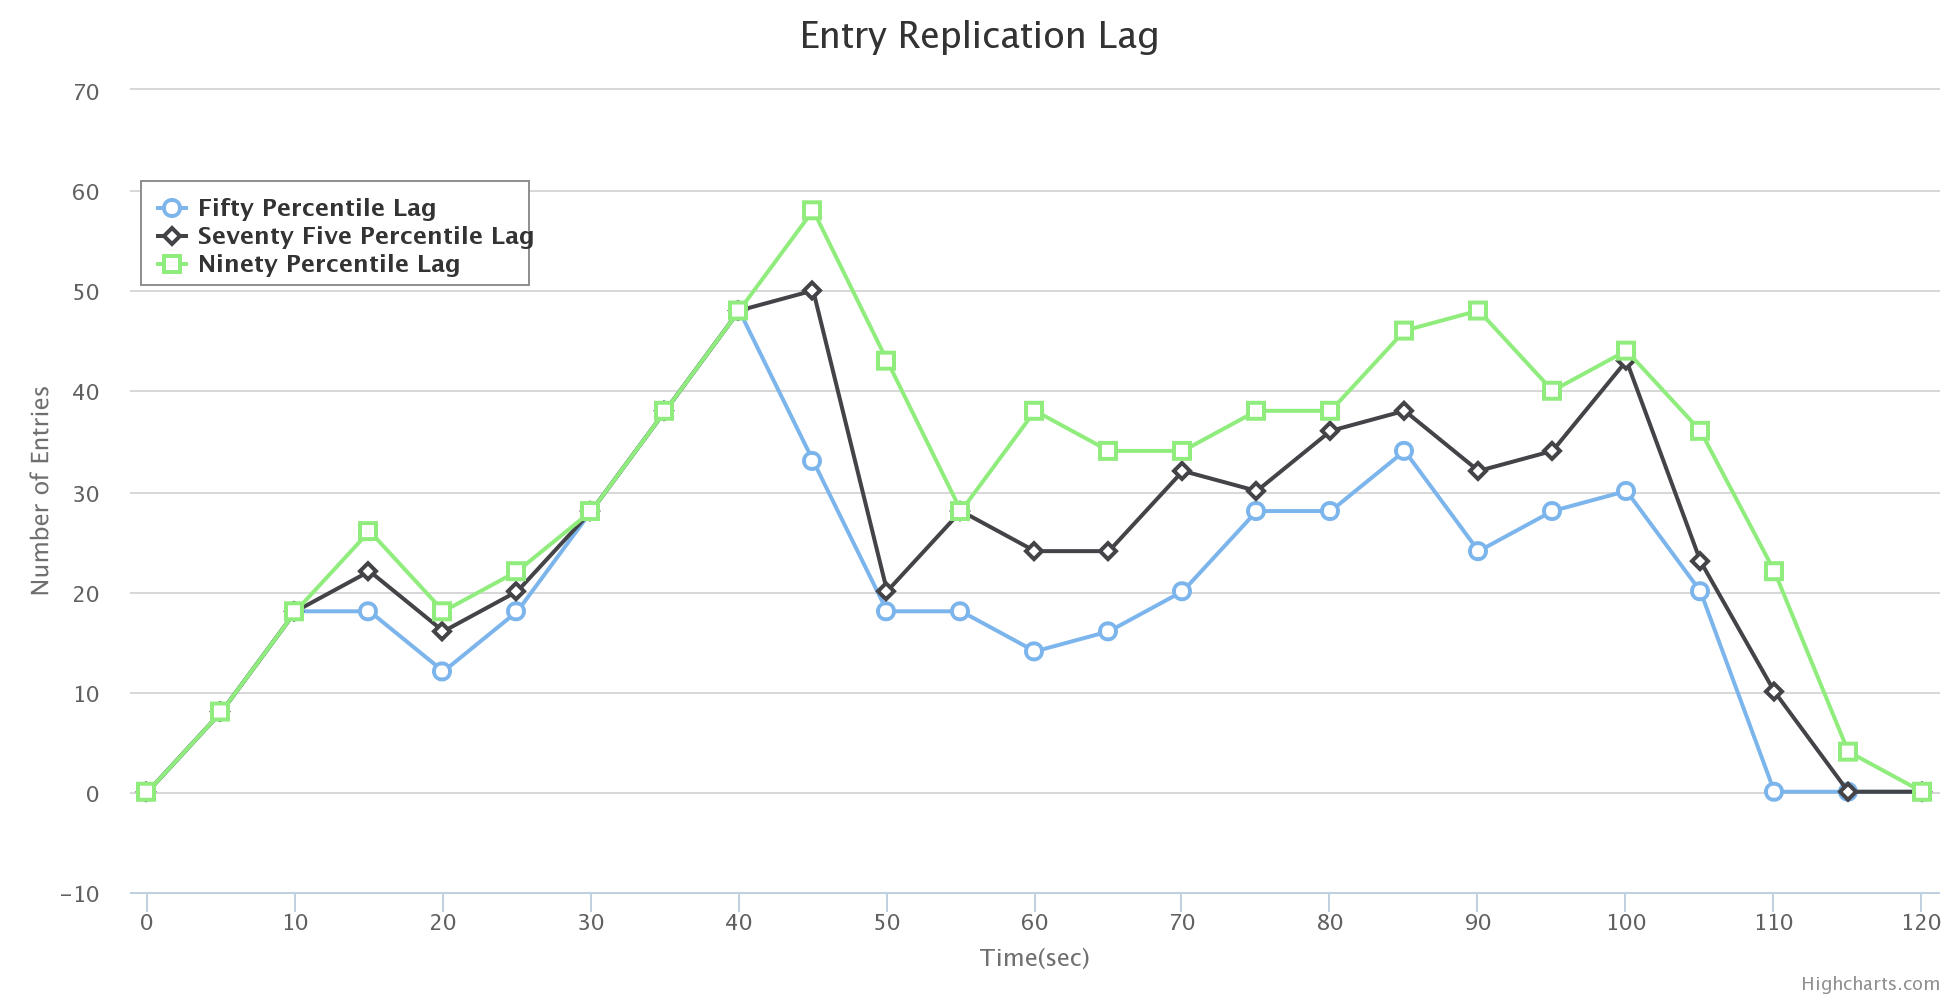
\includegraphics[scale=0.2]{Add200-2EntryPerSec}
	\caption{Add-Entry 2 entry(s)/Sec}
	\label{fig:addEntry2}
\end{figure}



\begin{figure}[h]
	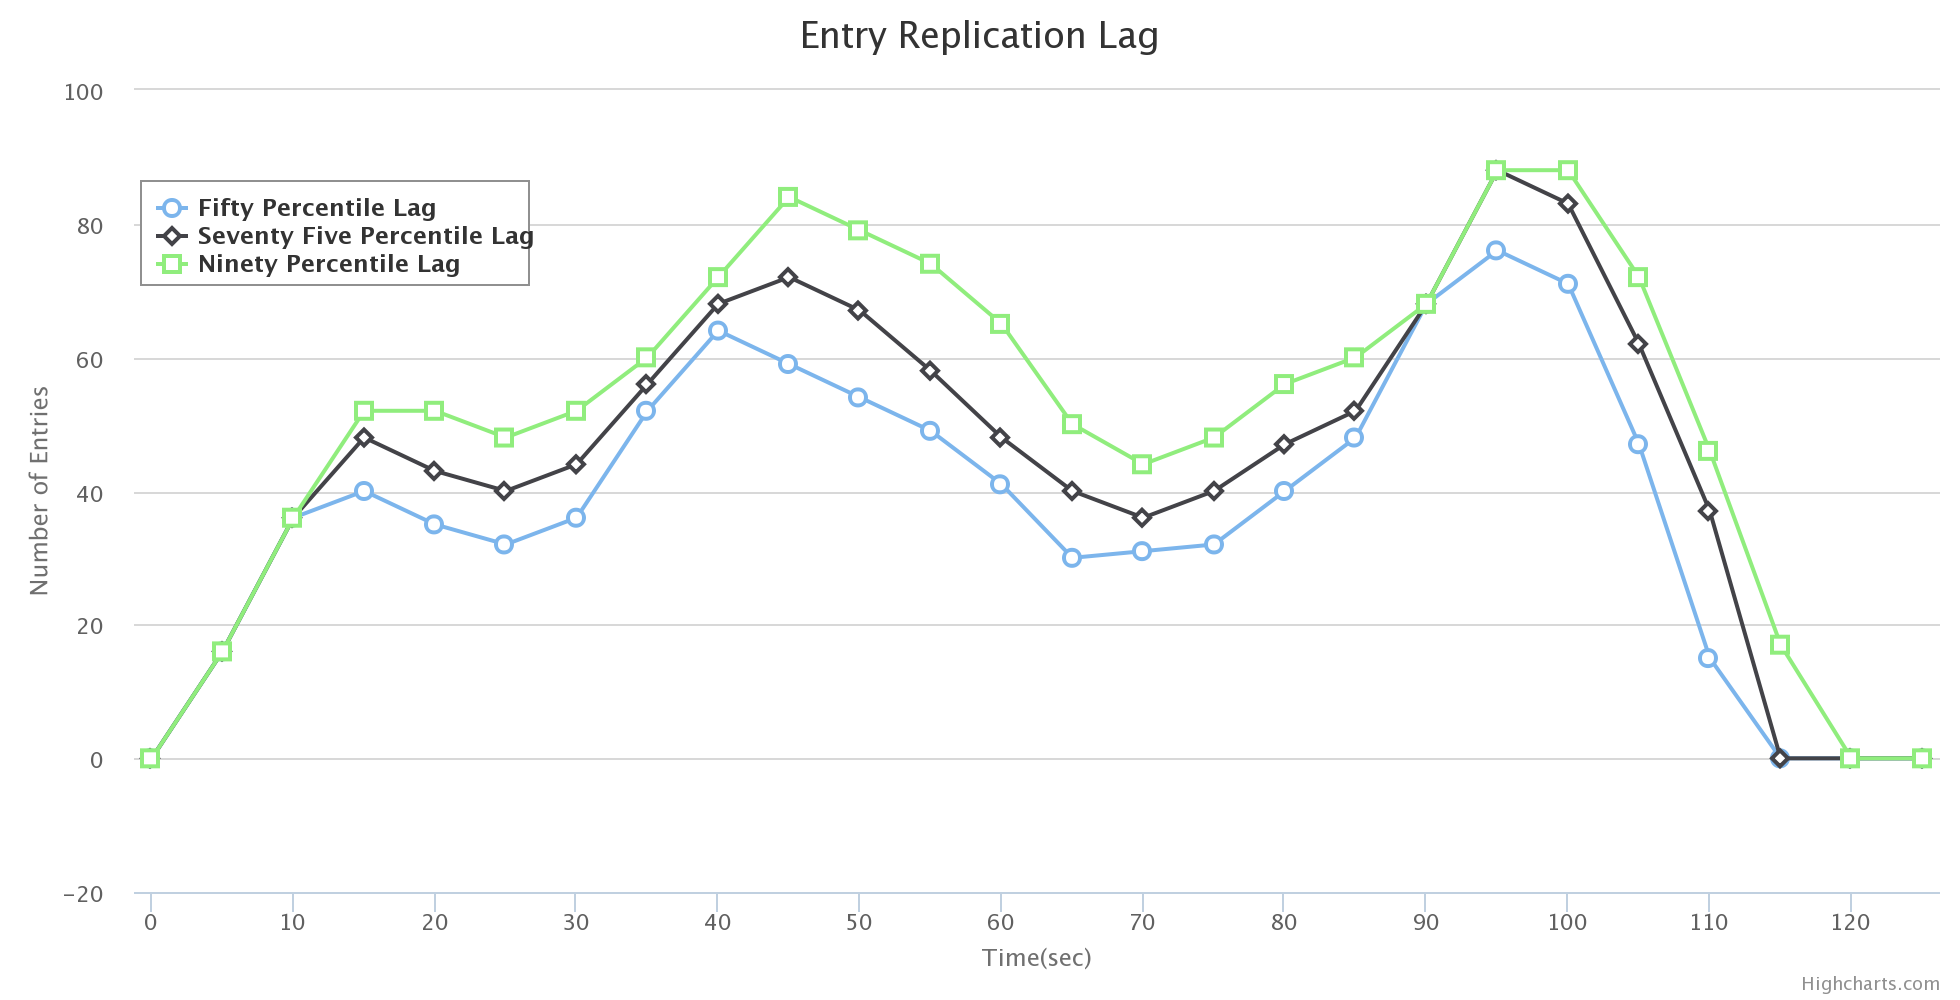
\includegraphics[scale=0.2]{Add200-4EntryPerSec}
	\caption{Add-Entry 4 entry(s)/Sec}
	\label{fig:addEntry4}
\end{figure}

\section{Churn Experiment}
\label{sec:churn}
As part of this experiment, we initialized the cluster with 200 nodes and once the system got stabilized we added \textit{100 entries} . We then, initiated the churn process in the system for a fixed period of time during which we added and simultaneously removed \textit{four nodes per sec} to and from the system respectively. Each node in the system except from the leader and the nodes in the follower group had an equal chance to be selected for the removal from the system. The process of removal involved shutting down the node and stopping all of its communication with other nodes. Once a node is removed, it is not allowed to join back in the system. The nodes added as part of churn process joined the system with a unique identifier. In addition to this, during the churn process, a constant rate of \textit{ One entry per sec} was employed for the entry addition. As part of the experiment, we tried to identify the maximum lag in the number of entries at different regions from center of the gradient. In ideal scenario, the lag at the center of the system i.e at the leader and its follower group is \textit{zero}. When we move away from the center of the gradient, the lag starts to increase as the nodes now need to identify and pull the latest information from the nodes above themselves. We tried to analyze the maximum lag in regions that are fifty percent, seventy five percent and ninety percent away from the center of the system. The results indicating the lag are shown in figure \ref{fig:churn}. The maximum lag as expected is in the outermost ring which is ninety percent away from the center of the system as the new nodes that are being added are present in that region due to very low utility. The fifty percent region remains stable, as the nodes nearby the center are able to quickly pull the updates and even though the nodes are being removed, the nodes from the outer regions move towards the inner regions eventually and fill the places of the crashed nodes. The system quickly recovers when the churn stops and lag eventually drops to \textit{zero}.

\begin{figure}[h]
	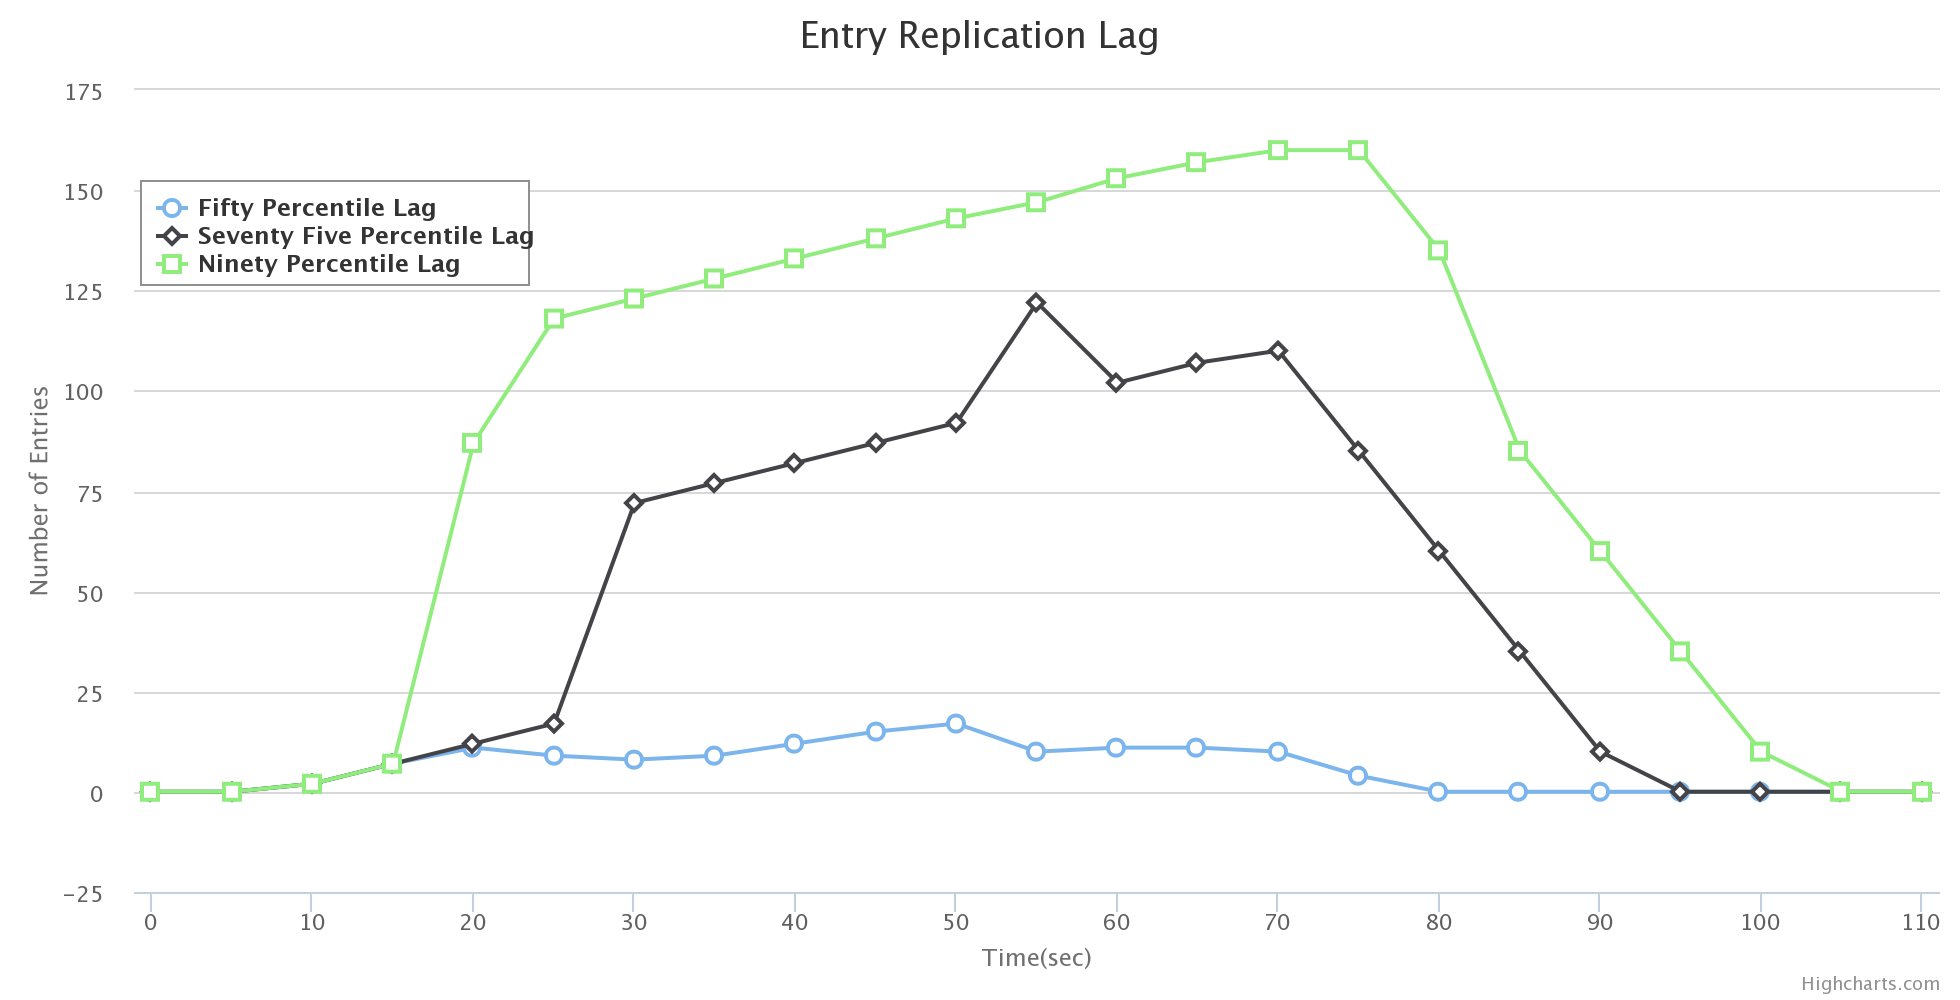
\includegraphics[scale=0.20]{Churn200-4Node-1Entry}
	\caption{Churn 4 nodes/sec and 1 entry/sec}
	\label{fig:churn}
\end{figure}

\section{Flash Crowd Experiment}
As part of this experiment we started with 200 nodes in the system and loaded the system initially with 100 entries. We then introduced a bunch of fresh nodes in the system in quick succession and analyzed the time it took for the nodes to catch up to the nodes already present in the system in terms of the entries already added to them. We performed the experiment for flash crowd size of \textit{10 percent, 20 percent and 40 percent} of the original nodes in the system. As we can see from Figure \ref{fig:flash40} and \ref{fig:flash80}, it it took the nodes approximately \textit{ 15 - 20 seconds} for the nodes to catch up in terms of having fifty percent of the entries with the nodes already present. In addition to this, the time taken by nodes to catch up with the seventy five and ninety nine of the entries is approximately in the same range.

\begin{figure}[h]
	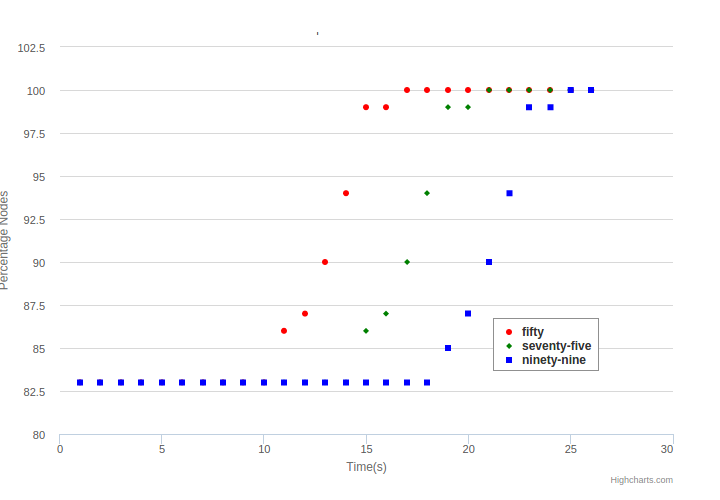
\includegraphics[scale=0.5]{200-40Nodes}
	\caption{FlashCrowd 40 nodes/Sec }
	\label{fig:flash40}
\end{figure}

\par Ideally as the \textit{maxEntryFetch} parameter per entry pull is \textit{twenty five}, it should take sixteen seconds i.e \textit{4 pull rounds} approximately for the nodes to fetch all the entries in the system but as observed from the diagram it takes more time than that. It is because it takes some time for the nodes to adjust themselves in the overall gradient and then pull the control information. Once the control information is pulled and verified, the nodes are able to determine the entries in the system at that moment and then start looking for the entries by requesting them from the nodes higher than themselves in terms of utility.

\begin{figure}[h]
	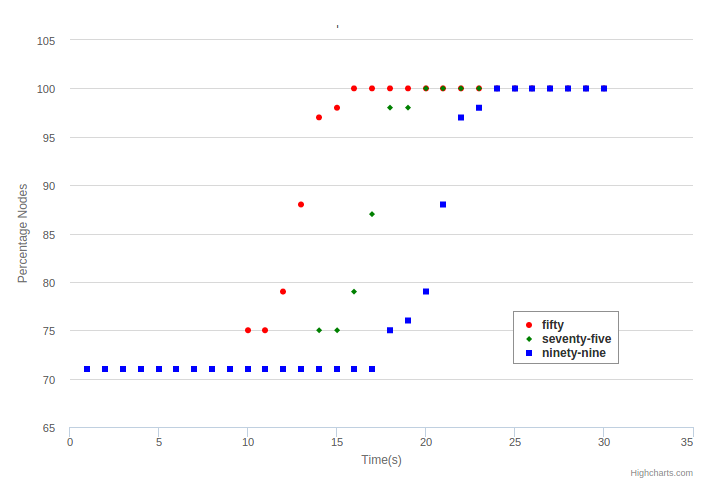
\includegraphics[scale=0.5]{200-80Nodes}
	\caption{FlashCrowd 80 nodes/Sec }
	\label{fig:flash80}
\end{figure}



\section{Flash Crowd and Churn Experiment}

In all of the above experiments, the system is analyzed based on a single scenario but in this experiment, we will be testing the system on multiple scenarios simultaneously. The cluster of nodes is initialized with \textit{100 entries}. Once the system becomes stable, we initiate a flashcrowd of \textit{forty nodes}. The initial spike as shown in Figure \ref{fig:flashChurn} depicts the sudden increase in the entry lag in the outermost ring in the system. Once the lag subsides, we initiate churn process similar to the one described in section  \ref{sec:churn}. In addition to this, we simultaneously initiate another flashcrowd by injecting \textit{twenty nodes} in the system. Before the lag caused by these fresh nodes subsides, we initiate a final flashcrowd of \textit{twenty nodes}. This effects of these events could be viewed in the series of sudden increase in the maximum lag in the seventy percentile region in the system. Even though the same pattern of increase in maximum lag is depicted in the fifty percentile region but the increase in the maximum lag is significantly less than in the outer regions indicating a higher stability in this region. 

\begin{figure}[h]
	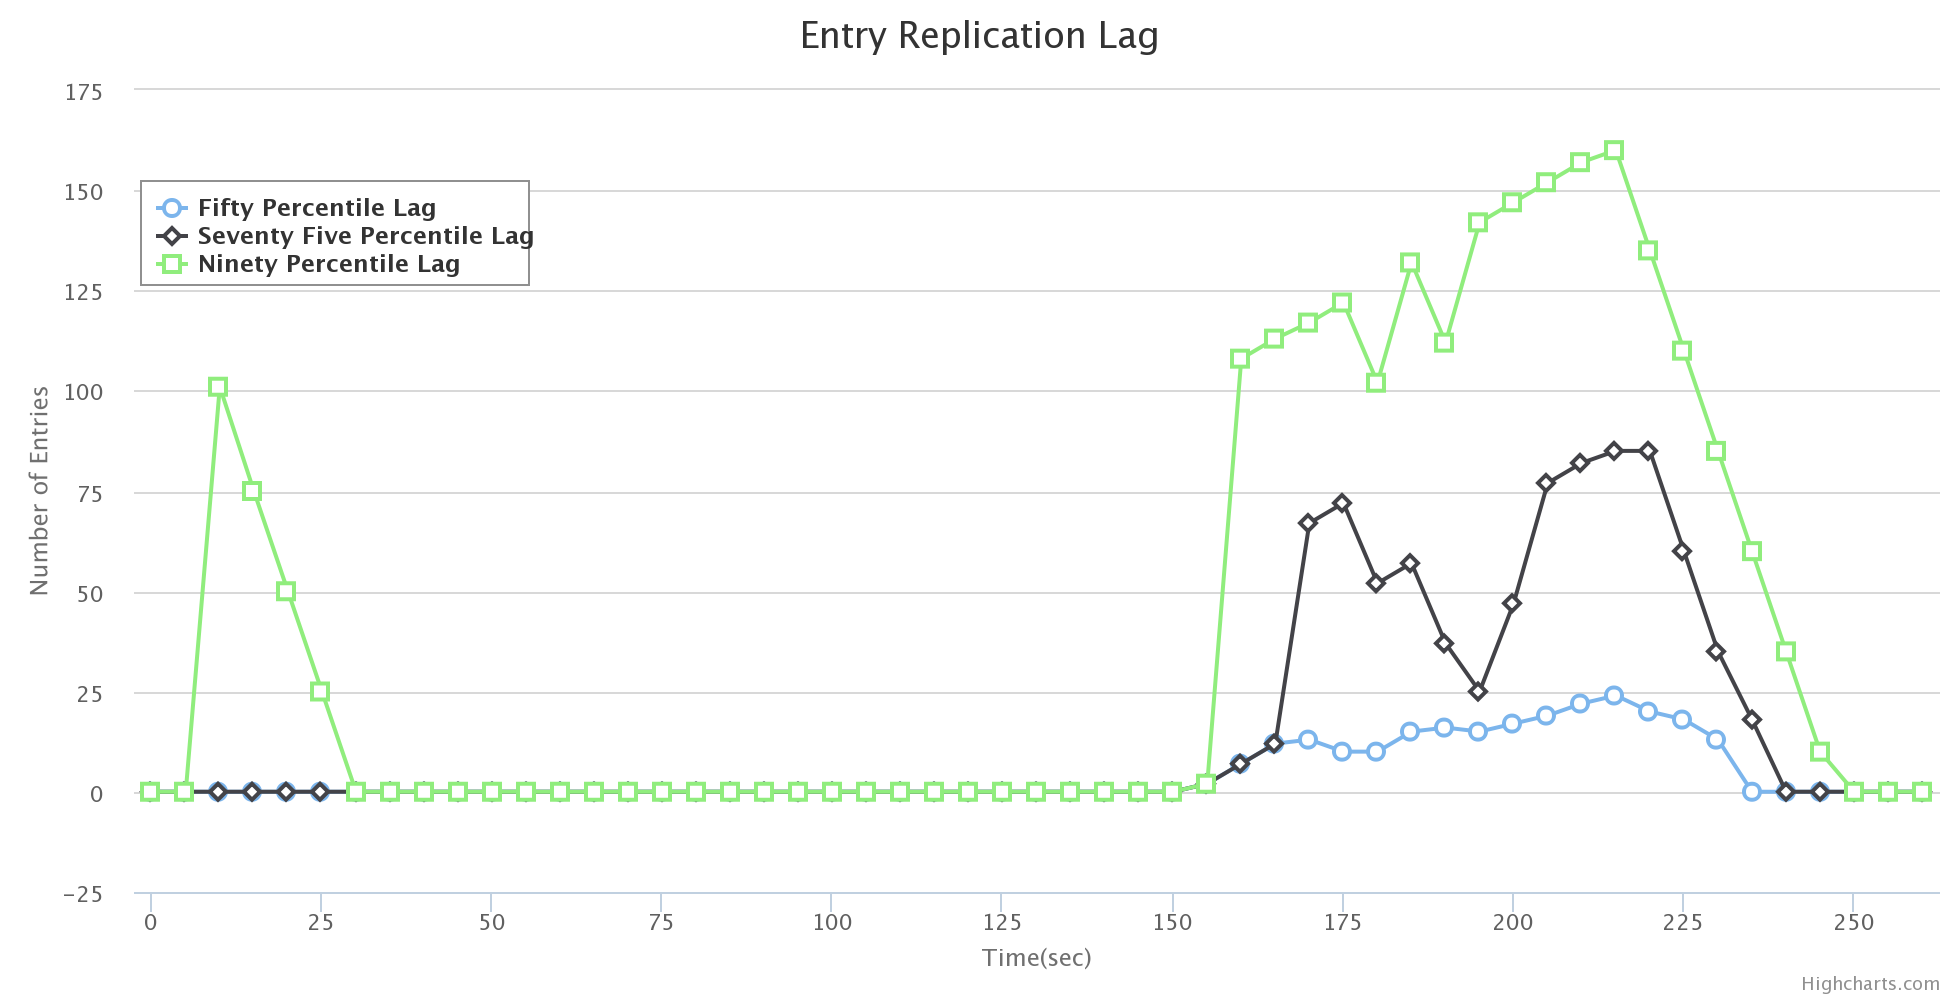
\includegraphics[scale=0.20]{Churn200-40Nodes-1-40-20-20}
	\caption{Churn and FlashCrowd}
	\label{fig:flashChurn}
\end{figure}



\chapter{Conclusion}
\label{chap:conclusion}

As part of thesis, we introduced the architecture and design behind a Full Text Decentralized Peer to Peer Search System. In addition to this, we also developed a prototype based on the mentioned principles. The prototype is built over the overlay which in turn is constructed using gradient topology. The topology uses a preference function to form links with the preferred nodes in the system. As part of prototype, each node prefers nodes with higher utility but closer to them. In addition to this, in order to help with the coordination among the nodes, we introduced a weaker form of leader election protocol known as Leader Selection. Each node base on its local utility and neighbors determines its claim to become a leader for a particular shard and if the criteria is fulfilled initiates voting protocol. A peer once chosen leader for shard identifies the followers which are group of nodes over which the operations carries out by leader will be replicated. Leader also initiates a lease, after which it has to re-ascertain itself as a leader, failing which the follower group will remove it from the leader position and wait for another leader to emerge.
\par The whole system which is composed of a number of shards, is controlled by a small and fixed number of peers which are the leaders and its follower group for every shard. The prototype at present, exposes \textit{ADD} and \textit{SEARCH} entry operations. For adding a new entry, the request is redirected to the leader of shard which then replicates it over the follower group. Each node then pulls the information from the nodes above in the utility resulting in dissemination of the information in the system. In order to search, the request is sent to a random node in all the shards. The requesting node then wait for the responses from each shard after which it replies back to the client with relevant information. This fanout of search request to multiple shards is affected by latency variability wherein a single slow running node in one of the shards will affect the total response time of the shard request. To prevent this, the request is sent to multiple nodes in each shard and only response from the fastest node from each shard is considered.

\section{Future work}
\label{sec:future-work}
%% What you have left undone?
%% What are the next obvious things to be done?
%% What hints can you give to the next person who is going to followup upon your work?

The thesis presents a prototype implementation for the full text decentralized search based on Apache Lucene. The future work for the prototype built is briefly explained in this section:


\subsection{Delete and Update Operations}

As part of the implementation, the system only deals with the \textit{Add} and \textit{Search} entry operations. This greatly simplifies the execution as the entries are not modifiable and therefore the client needs to add a new entry with the updated values. In future, we would like to provide the user with update operation in which the application will still create a new entry to be added in the system but will delete the previous entry. The delete entry operation is difficult to implement because of the fact that the entry gets replicated to all the nodes in the system through the pull protocol. In order to implement a delete operation a special entry needs to be committed by the leader which would need to be pulled by the nodes in the shard and which will indicate delete operation for a particular entry from the datastore.

\subsection{Server Side Pagination}

Whenever a client initiates a search request, the number of matches for a particular search query could be very large. Sending all the data every time a search query is initiated can overwhelm the network. As part of current prototype implementation, to keep things simple we reply back with all the data matching the search query. In future as the amount of data in system will grow, this approach will become unfeasible. Therefore we would need to implement server side pagination, where in the client will generate the search request and send it to the server. The search request will also contain the page number and number of results which will enable the server to execute the query and sort the results and only return the results that would lie in that particular page number. If clients wont to see more responses, they will again initiate the same query but with a different page number to the server.


\subsection{Edge Case Identification}

As the system is asynchronous and composed of various components, each working independently of the other, certain edge cases exists for which the handling has not been defined. The priority will be to identify these cases and then handle them correctly. In addition to this, semantics of the fault handling and resolution is not defined yet. For now, in case of a fault like unable to write to data storage or individual components crashing, we simply throw an exception and crash the peer. This results in a poor user experience and therefore better fault handling and resolution needs to be carried out.


\subsection{Robust Sharding Protocol}
At present, the leader generates the splitting point and then each node based on the bitwise manipulation algorithm applied on its self identifier, decides to either remove the leader units above the splitting point or below it. This is a very basic approach. In future we would like to implement another bitwise manipulation algorithm which based on the metadata for each leader unit would identify the location of each leader unit after sharding. In this way the units could be transferred in different shards. The only drawback is that it would result in imbalance in load as it might be possible that the units identified to be sent to a particular shard have very less entries that the other ones meaning all the low capacity leader units might go in one shard and high capacity units in another shard. This problem needs to be solved before switching to the approach mentioned in this section.




\bibliography{report}
\bibliographystyle{IEEEtran}
%%\bibliographystyle{unsrturl}
%%\bibliographystyle{unsrtnat}
%%\bibliographystyle{myIEEEtran}
\appendix
%\chapter{Insensible Approximation}

%\backmatter

\end{document}
